%
% Template Laporan Skripsi/Thesis 
%
% @author  Andreas Febrian, Lia Sadita 
% @version 1.03
%
% Dokumen ini dibuat berdasarkan standar IEEE dalam membuat class untuk 
% LaTeX dan konfigurasi LaTeX yang digunakan Fahrurrozi Rahman ketika 
% membuat laporan skripsi. Konfigurasi yang lama telah disesuaikan dengan 
% aturan penulisan thesis yang dikeluarkan UI pada tahun 2008.
%

%
% Tipe dokumen adalah report dengan satu kolom. 
%
\documentclass[12pt, a4paper, onecolumn, oneside, final]{report}

% Load konfigurasi LaTeX untuk tipe laporan thesis
\usepackage{uithesis}
\usepackage[ruled,vlined]{algorithm2e}


% Load konfigurasi khusus untuk laporan yang sedang dibuat
%-----------------------------------------------------------------------------%
% Informasi Mengenai Dokumen
%-----------------------------------------------------------------------------%
% 
% Judul laporan. 
\var{\judul}{Metode Seleksi Fitur Berbasis Perankingan Bobot Secara Multi Step Menggunakan Deep Learning untuk Pencarian Biomarker pada Data Microarray}
% 
% Tulis kembali judul laporan, kali ini akan diubah menjadi huruf kapital
\Var{\Judul}{Metode Seleksi Fitur Berbasis Perankingan Bobot Secara Multi Step Menggunakan Deep Learning untuk Pencarian Biomarker pada Data Microarray}
% 
% Tulis kembali judul laporan namun dengan bahasa Ingris
\var{\judulInggris}{FEATURE SELECTION METHOD BASED ON MULTI STEP WEIGHT RANKING USING DEEP LEARNING TO SEARCH BIOMARKER IN LUNG CANCER MICROARRAY DATA SET}

% 
% Tipe laporan, dapat berisi Skripsi, Tugas Akhir, Thesis, atau Disertasi
\var{\type}{Thesis}
% 
% Tulis kembali tipe laporan, kali ini akan diubah menjadi huruf kapital
\Var{\Type}{Thesis}
% 
% Tulis nama penulis 
\var{\penulis}{Mukhlis Amien}
% 
% Tulis kembali nama penulis, kali ini akan diubah menjadi huruf kapital
\Var{\Penulis}{Mukhlis Amien}
% 
% Tulis NPM penulis
\var{\npm}{1406522102}
% 
% Tuliskan Fakultas dimana penulis berada
\Var{\Fakultas}{Ilmu Komputer}
\var{\fakultas}{Ilmu Komputer}
% 
% Tuliskan Program Studi yang diambil penulis
\Var{\Program}{Magister Ilmu Komputer}
\var{\program}{Magister Ilmu Komputer}
% 
% Tuliskan tahun publikasi laporan
\Var{\bulanTahun}{Juni 2016}
% 
% Tuliskan gelar yang akan diperoleh dengan menyerahkan laporan ini
\var{\gelar}{Master}
% 
% Tuliskan tanggal pengesahan laporan, waktu dimana laporan diserahkan ke 
% penguji/sekretariat
\var{\tanggalPengesahan}{20 Juni 2016} 
% 
% Tuliskan tanggal keputusan sidang dikeluarkan dan penulis dinyatakan 
% lulus/tidak lulus
\var{\tanggalLulus}{XX Juni 2016}
% 
% Tuliskan pembimbing 
\var{\pembimbing}{Ito Wasito PhD.}
% 
% Alias untuk memudahkan alur penulisan paa saat menulis laporan
\var{\saya}{Mukhlis Amien}

%-----------------------------------------------------------------------------%
% Judul Setiap Bab
%-----------------------------------------------------------------------------%
% 
% Berikut ada judul-judul setiap bab. 
% Silahkan diubah sesuai dengan kebutuhan. 
% 
\Var{\kataPengantar}{Kata Pengantar}
\Var{\babSatu}{Pendahuluan}
\Var{\babDua}{Tinjauan Pustaka}
\Var{\babTiga}{Metodologi Penelitian}
\Var{\babEmpat}{Pembahasan}
\Var{\kesimpulan}{Kesimpulan dan Saran}

% Daftar pemenggalan suku kata dan istilah dalam LaTeX
%
% Hyphenation untuk Indonesia 
%
% @author  Andreas Febrian
% @version 1.00
% 
% Tambahkan cara pemenggalan kata-kata yang salah dipenggal secara otomatis 
% oleh LaTeX. Jika kata tersebut dapat dipenggal dengan benar, maka tidak 
% perlu ditambahkan dalam berkas ini. Tanda pemenggalan kata menggunakan 
% tanda '-'; contoh:
% menarik
%   --> pemenggalan: me-na-rik
%

\hyphenation{
    % alphabhet A
    a-na-li-sa a-tur 
    a-pli-ka-si 
    % alphabhet B
    ba-ngun-an 
    be-be-ra-pa 
    ber-ge-rak
    ber-ke-lan-jut-an 
    ber-pe-nga-ruh 
    % alphabhet C
    ca-ri
    % alphabhet D
    di-sim-pan di-pim-pin de-ngan da-e-rah di-ba-ngun da-pat di-nya-ta-kan 
    di-sim-bol-kan di-pi-lih di-li-hat de-fi-ni-si
    % alphabhet E
    e-ner-gi eks-klu-sif
    % alphabhet F
    fa-si-li-tas
    % alphabhet G
    ga-bung-an ge-rak
    % alphabhet H
    ha-lang-an
    % alphabhet I
    % alphabhet J
    % alphabhet K
    ke-hi-lang-an
    ku-ning 
    kua-li-tas ka-me-ra ke-mung-kin-an ke-se-pa-ham-an
    % alphabhet L
    ling-kung-an
    % alphabhet M
    me-neng-ah
    meng-a-tas-i me-mung-kin-kan me-nge-na-i me-ngi-rim-kan 
    meng-u-bah meng-a-dap-ta-si me-nya-ta-kan mo-di-fi-ka-si
    meng-a-tur
    % alphabhet N
    nya-ta non-eks-klu-sif
    % alphabhet O
    % alphabhet P
	pe-nye-rap-an 
	pe-ngon-trol
    pe-mo-del-an
    pe-ran  pe-ran-an-nya
    pem-ba-ngun-an pre-si-den pe-me-rin-tah prio-ri-tas peng-am-bil-an 
    peng-ga-bung-an pe-nga-was-an pe-ngem-bang-an 
    pe-nga-ruh pa-ra-lel-is-me per-hi-tung-an per-ma-sa-lah-an 
    pen-ca-ri-an peng-struk-tur-an
    % alphabhet Q
    % alphabhet R
    ran-cang-an
    % alphabhet S
    si-mu-la-si sa-ngat
    % alphabhet T
    te-ngah
    ter-da-pat
    % alphabhet U
    % alphabhet V
    % alphabhet W
    % alphabhet X
    % alphabhet Y
    % alphabhet Z
    % special
}
% Daftar istilah yang mungkin perlu ditandai 
%
% @author  Andreas Febrian
% @version 1.00
% 
% Mendaftar seluruh istilah yang mungkin akan perlu dijadikan 
% italic atau bold pada setiap kemunculannya dalam dokumen. 
% 

\var{\license}{\f{Creative Common License 1.0 Generic}}
\var{\bslash}{$\setminus$}

% Awal bagian penulisan laporan
\begin{document}
%
% Sampul Laporan
%
% Sampul Laporan

%
% @author  unknown
% @version 1.01
% @edit by Andreas Febrian
%

\begin{titlepage}
    \begin{center}    
        \begin{figure}
            \begin{center}
                
\includegraphics[width=2.5cm]{pics/makara.png}
            \end{center}
        \end{figure}    
        \vspace*{0cm}
        \bo{
        	UNIVERSITAS INDONESIA\\
        }
        
        \vspace*{1.0cm}
        % judul thesis harus dalam 14pt Times New Roman
        \bo{\Judul} \\[1.0cm]

        \vspace*{2.5 cm}    
        % harus dalam 14pt Times New Roman
        \bo{\Type}

        \vspace*{3 cm}       
        % penulis dan npm
        \bo{\Penulis} \\
        \bo{\npm} \\

        \vspace*{5.0cm}

        % informasi mengenai fakultas dan program studi
        \bo{
        	FAKULTAS \Fakultas\\
        	PROGRAM STUDI \Program \\
        	DEPOK \\
        	\bulanTahun
        }
    \end{center}
\end{titlepage}


%
% Gunakan penomeran romawi
\pagenumbering{roman}

%
% load halaman judul dalam
\addChapter{HALAMAN JUDUL}
%
% Halaman Judul Laporan 
%
% @author  unknown
% @version 1.01
% @edit by Andreas Febrian
%

\begin{titlepage}
    \begin{center}\begin{figure}
            \begin{center}
                
\includegraphics[width=2.5cm]{pics/makara.png}
            \end{center}
        \end{figure}    
        \vspace*{0cm}
        \bo{
        	UNIVERSITAS INDONESIA\\
        }
        
        \vspace*{1.0cm}
        % judul thesis harus dalam 14pt Times New Roman
        \bo{\Judul} \\[1.0cm]

        \vspace*{2.5 cm}    
        % harus dalam 14pt Times New Roman
        \bo{\Type} \\
        % keterangan prasyarat
        \bo{Diajukan sebagai salah satu syarat untuk memperoleh gelar \\
        \gelar}\\

        \vspace*{3 cm}       
        % penulis dan npm
        \bo{\Penulis} \\
        \bo{\npm} \\

        \vspace*{5.0cm}

        % informasi mengenai fakultas dan program studi
        \bo{
        	FAKULTAS \Fakultas\\
        	PROGRAM STUDI \Program \\
        	DEPOK \\
        	\bulanTahun
        }
    \end{center}
\end{titlepage}

%
% setelah bagian ini, halaman dihitung sebagai halaman ke 2
\setcounter{page}{2}

%
% load halaman pengesahan
\addChapter{LEMBAR PERSETUJUAN}
%
% Halaman Pengesahan
%
% @author  Andreas Febrian
% @version 1.01
%

\chapter*{HALAMAN PERSETUJUAN}

\vspace*{0.2cm}
\noindent 

\noindent
\begin{tabular}{l l p{11cm}}
	\bo{Judul}&: & \judul \\ 
	\bo{Nama}&: & \penulis \\
	\bo{NPM}&: & \npm \\
\end{tabular} \\

\vspace*{1.2cm}

\noindent Laporan \type~ini telah diperiksa dan disetujui.\\[0.3cm]
\begin{center}
\tanggalPengesahan \\[2cm]


\underline{\pembimbing}\\[0.1cm]
Pembimbing \type
\end{center}

\newpage
%
% load halaman orisinalitas 
\addChapter{LEMBAR PERNYATAAN ORISINALITAS}
%
% Halaman Orisinalitas
%
% @author  Andreas Febrian
% @version 1.01
%

\chapter*{\uppercase{halaman pernyataan orisinalitas}}
\vspace*{2cm}

\begin{center}
	\bo{\type~ini adalah hasil karya saya sendiri, \\ 
	dan semua sumber baik yang dikutip maupun dirujuk \\
	telah saya nyatakan dengan benar.} \\
	\vspace*{2.6cm}
	
	\begin{tabular}{l c l}
	\bo{Nama} & : & \bo{\penulis} \\
	\bo{NPM} & : & \bo{\npm} \\ 
	\bo{Tanda Tangan} & : & \\
	& & \\
	& & \\
	\bo{Tanggal} & : & \bo{\tanggalPengesahan} \\	
	\end{tabular}
\end{center}

\newpage
%
%
\addChapter{LEMBAR PENGESAHAN}
%
% Halaman Pengesahan Sidang
%
% @author  Andreas Febrian, Andre Tampubolon 
% @version 1.02
%

\chapter*{HALAMAN PENGESAHAN}

\vspace*{0.4cm}
\noindent 

\noindent
\begin{tabular}{ll p{9cm}}
	\type~ini diajukan oleh&: & \\
	Nama&: & \penulis \\
	NPM&: & \npm \\
	Program Studi&: & \program \\
	Judul \type&: & \judul \\
\end{tabular} \\

\vspace*{1.0cm}

\noindent \bo{Telah berhasil dipertahankan di hadapan Dewan Penguji 
dan diterima sebagai bagian persyaratan yang diperlukan untuk 
memperoleh gelar \gelar~pada Program Studi \program, Fakultas 
\fakultas, Universitas Indonesia.}\\[0.2cm]

\begin{center}
	\bo{DEWAN PENGUJI}
\end{center}

\vspace*{0.3cm}

\begin{tabular}{l l l l }
	& & & \\
	Pembimbing&: & \pembimbing & (\hspace*{3.0cm}) \\
	& & & \\
	Penguji&: & Ari Saptawijaya, S.Kom., M.Sc., Ph.D. & (\hspace*{3.0cm}) \\
	& & & \\
	Penguji&: & dr. Iik Wilarso M.T.I. & (\hspace*{3.0cm}) \\
	& & & \\
	Penguji&: & Dr. Eng. M. Rahmat Widyanto S.Kom., M.Eng. & (\hspace*{3.0cm}) \\
\end{tabular}\\



\vspace*{2.0cm}

\begin{tabular}{ll l}
	Ditetapkan di&: & Depok\\
	Tanggal&: & \tanggalLulus \\
\end{tabular}


\newpage
%
%
\addChapter{\kataPengantar}
%-----------------------------------------------------------------------------%
\chapter*{\kataPengantar}
%-----------------------------------------------------------------------------%
Pertama-tama saya ucapkan puji syukur kehadirat Allah SWT dan Junjungan kita Nabi Muhammad SAW, atas segala karunianya-lah thesis ini bisa terselesaikan. Saya mengucapkan terima kasih yang sebesar-besarnya atas bimbingan yang diberikan oleh dosen pembimbing saya Bapak Ir. Ito Wasito M.Sc, Ph.D. Kepada istri saya, Catur Prastiasih yang sangat mendukung  saya melanjutkan sekolah. Kepada teman-teman satu bimbingan yaitu Aries dan Arida yang telah memberikan ide, masukan dan diskusi yang mendalam. \\
Kepada Fakultas Ilmu Komputer Universitas Indonesia, yang telah memberikan fasilitas lab yang sangat membantu saya dalam menyelesaikan thesis ini. \\
Kepada orang tua saya, terima-kasih banyak atas dukungan moral dan spiritual yang diberikan. Dan saudara-saudara saya di Batu.

\vspace*{0.1cm}
\begin{flushright}
Depok, 20 Juni 2016\\[0.1cm]
\vspace*{1cm}
\penulis

\end{flushright}
%
%
\addChapter{LEMBAR PERSETUJUAN PUBLIKASI ILMIAH}
% 
% @author  Andre Tampubolon, Andreas Febrian
% @version 1.01
% 

\chapter*{\uppercase{Halaman Pernyataan Persetujuan Publikasi Tugas Akhir untuk Kepentingan Akademis}}

\vspace*{0.2cm}
\noindent 
Sebagai sivitas akademik Universitas Indonesia, saya yang bertanda 
tangan di bawah ini:
\vspace*{0.4cm}


\begin{tabular}{p{4.2cm} l p{6cm}}
	\bo{Nama} & : & \penulis \\ 	
	\bo{NPM} & : & \npm \\
	\bo{Program Studi} & : & \program\\	
	\bo{Fakultas} & : & \fakultas\\
	\bo{Jenis Karya} & : & \type \\
\end{tabular}

\vspace*{0.6cm}
\noindent demi pengembangan ilmu pengetahuan, menyetujui untuk memberikan 
kepada Universitas Indonesia \bo{Hak Bebas Royalti Noneksklusif 
(Non-exclusive Royalty Free Right)} atas karya ilmiah saya yang berjudul:
\begin{center}
	\judul
\end{center}
beserta perangkat yang ada (jika diperlukan). Dengan Hak Bebas Royalti 
Noneksklusif ini Universitas Indonesia berhak menyimpan, 
mengalihmedia/formatkan, mengelola dalam bentuk pangkalan data 
(database), merawat, dan memublikasikan tugas akhir saya selama 
tetap mencantumkan nama saya sebagai penulis/pencipta dan sebagai 
pemilik Hak Cipta. \\

\noindent Demikian pernyatan ini saya buat dengan sebenarnya.

\begin{center}
	\vspace*{0.8cm}
	\begin{tabular}{lll}
		Dibuat di&: & Depok \\
		Pada tanggal&: & \tanggalPengesahan \\
	\end{tabular}\\

	\vspace*{0.2cm}
	Yang menyatakan \\
	\vspace*{1.1cm}
	(\penulis)
\end{center}

\newpage


%
% 
\addChapter{ABSTRAK}
%
% Halaman Abstrak
%
% @author  Andreas Febrian
% @version 1.00
%

\chapter*{Abstrak}

\vspace*{0.2cm}

\noindent \begin{tabular}{l l p{10cm}}
	Nama&: & \penulis \\
	Program Studi&: & \program \\
	Judul&: & \judul \\
\end{tabular} \\ 

\vspace*{0.5cm}

\noindent 
Data ekspresi gen pada percobaan microarray memiliki ciri khas yaitu jumlah sampel yang sedikit dengan dimensi fitur yang sangat besar. Algoritma \textit{Deep Believe Network (DBN)}  adalah bagian dari algoritma \textit{deep learning} yang menerapkan teknik \textit{unsupervised learning}, digunakan untuk membantu menganalisa data ekspresi gen. Algoritma seleksi fitur yang berbasis pada perankingan bobot secara multi-step digunakan untuk mendapatkan fitur gen yang paling penting. Pemilihan fitur yang paling informatif dari suatu kasus percobaan microarray, merupakan  masalah yang ada pada pemrosesan data ekspresi gen. Sehingga diperlukan eksplorasi lebih lanjut untuk pemilihan fiturnya. Seleksi fitur gen, berdasarkan ranking bobot yang dihasilkan oleh \textit{deep learning}, diharapkan dapat memecahkan masalah seleksi fitur tersebut. Sedangkan metode clustering yang dipakai adalah: Cluster Affinity Search Technique (CAST) , K-Means Clustering dan Hierarchical Clustering. Deep learning adalah metode pembelajaran mesin yang merupakan bagian dari algoritma neural network, metode deep learning yang sering dipakai adalah arsitektur deep believe network (DBN). Pendekatan unsupervised learning pada deep learning dan clustering, diharapkan dapat digunakan untuk membantu peneliti dalam menganalisa data ekspresi gen-nya.

\vspace*{0.2cm}

\noindent Kata Kunci: \\ 
\noindent 
\textit{Microarray, ekspresi gen, Algoritma Clustering, feature selection, deep learning, unsupervised learning.}

\newpage
%
%
%
% Halaman Abstract
%
% @author  Andreas Febrian
% @version 1.00
%

\chapter*{ABSTRACT}

\vspace*{0.2cm}

\noindent \begin{tabular}{l l p{11.0cm}}
	Name&: & \penulis \\
	Program&: & \program \\
	Title&: & \judulInggris \\
\end{tabular} \\ 

\vspace*{0.5cm}

\noindent 
Microarray technology has made possible the profiling of gene expressions of the entire genome in a single hybridization experiment. Since microarray data acquire tens of thousands of gene expression values simultaneously. However, the number of sample usually small. Feature selection and clustering algorithm for microarray data analysis is useful to extract cluster structure and to reduce the high dimensional microarray data and reconstruct to lower dimensional with minimum error possible. Deep learning and clustering is a machine learning method. In this research we will investigate the effectiveness of clustering after or prior dimensionality reduction. The most common deep learning architecture used for dimensionality reduction is deep believe network (DBN) and stacked auto encoder (SAE). Pre training unsupervised learning and greedy layer wise training approach are expected for better dimensionality reduction in microarray datasets compared with other methods.

\vspace*{0.2cm}

\noindent Keywords: \\ 
\noindent \textit{Microarray, ekspresi gen, Algoritma Clustering, feature selection, deep learning, unsupervised learning.}

\newpage

%
% Daftar isi, gambar, dan tabel
%
\tableofcontents
\clearpage
\listoffigures
\clearpage
\listoftables
\clearpage

%
% Gunakan penomeran Arab (1, 2, 3, ...) setelah bagian ini.
%
\pagenumbering{arabic}

%
%
%
%-----------------------------------------------------------------------------%
\chapter{\babSatu}
%-----------------------------------------------------------------------------%

%-----------------------------------------------------------------------------%
\section{Latar Belakang}
%-----------------------------------------------------------------------------%
Data ekspresi gen pada percobaan \textit{microarray} memiliki ciri khas yaitu dimensi fitur gen yang jauh lebih besar dibandingkan dengan sampel pasien yang sedikit dikarenakan oleh mahalnya percobaan dan terbatasnya pasien. Hal ini menyebabkan masalah pada penerapan teknik machine learning untuk pengenalan pola penyakit yang diinginkan. Oleh karena itu, dalam menyederhanakan data ekspresi gen tersebut, dibutuhkan metode seleksi fitur untuk mempermudah melakukan analisa gen dengan menyeleksi gen-gen yang dibutuhkan saja. \citep{yoon2006building}. Menurut penelitian \cite{yoon2006building} dan \cite{bandyopadhyay2014survey} tidak semua gen yang didapat dari percobaan microarray tersebut adalah gen yang informatif, bahkan jumlah ekspresi gen yang informatif untuk kasus yang diinginkan misalnya untuk pengenalan sel kanker, sangat sedikit dibandingkan dengan keseluruhan ekspresi gen yang didapat dalam sebuah eksperimen \citep{bandyopadhyay2014survey}. Data ekspresi gen yang tidak informatif tersebut dapat mengurangi performa  proses pengenalan pola secara signifikan pada teknik \textit{machine learning} yang diterapkan. Akan tetapi, beberapa gen yang informatif berpengaruh secara signifikan terhadap pengenalan pola tersebut. Sebagai contoh, untuk mendiagnosa kanker paru-paru, hanya dibutuhkan sekitar 50 gen saja dari 22 ribu gen yang didapatkan dalam percobaan. Gen-gen yang paling informatif ini disebut dengan Biomarker \citep{belinsky2004gene}. Sehingga, hanya dengan menggunakan data biomarker yang ditemukan, bisa dikenali penyakit yang diderita oleh pasien.\\
pengetahuan manusia tentang gen sampai saat ini masih terbatas, yaitu ada sekitar 26\% dari keseluruhan gen yang belum diketahui kegunaannya \citep{haggstrom2014diagram}. Oleh karena itu pendekatan teknik machine learning secara unsupervised sering dilakukan untuk analisa pengenalan pola data microarray. Pada penelitian ini, akan dilakukan seleksi fitur terhadap data microarray secara unsupervised learning dengan menggunakan teknik deep learning. Dari hasil seleksi fitur gen tersebut akan diterapkan algoritma supervised learning yang digunakan untuk melakukan evaluasi seberapa baik keakurasian seleksi fitur tersebut dalam pengenalan pola pendeteksian penyakit kanker paru-paru pada sample pasien sakit dan normal. \\
Untuk teknik seleksi fitur tersebut akan digunakan metode dengan cara melakukan modifikasi algoritma seleksi fitur untuk logistic regression dilakukan oleh \cite{shevade2003simple}. 
\todo{bagian bawah ini masih ruwet}
Dikarenakan algoritma seleksi fitur menggunakan logistic regression merupakan bagian dari supervised learning dan linier, maka dianggap kurang cocok untuk data microarray yang fungsinya belum diketahui secara lengkap dan memiliki karakteristik yang kompleks. Dan logistic regression memiliki masalah dalam  mengeliminasi fitur, dikarenakan koefisien bobot ditempatkan disetiap fitur. Oleh karena itu, disini akan diajukan arsitektur deep learning.
Arsitektur deep learning, yang akan digunakan pada penelitian ini adalah arsitektur Deep Belief Network (DBN). DBN merupakan jaringan Restrictive Boltzmann Machine (RBM) yang dijajarkan. Dimulai dengan memberikan bobot random diantara dua network, yang dapat di latih dengan cara meminimalkan perbedaan antara data asli dengan data rekonstruksinya. Gradien didapatkan dengan chain rule untuk melakukan penurunan error dengan teknik Contrastive Divergence (CD). Untuk dicari bobot (W) dengan maximum likelihood learning  secara greedy per layer-nya (greedy layer wise training) (Hinton, 2006). Pada penelitian ini, untuk mencari perangkingan bobotnya, menggunakan modifikasi dari cara yang digunakan oleh Shevade (Shevade, 2003) dalam teknik seleksi fitur berbasis weight menggunakan Sparse logistic regression (Shevade, 2003). Sehingga teori perankingan weight ini akan dimodifikasi dan digunakan untuk  meranking fiturnya secara multi step yang akan diterapkan pada DBN.
Tahap selanjutnya fitur yang telah didapatkan pada tahap seleksi fitur, akan digunakan sebagai data untuk penerapan clustering. Algoritma yang akan dipakai adalah : Cluster Affinity Search Technique (CAST) , K-Means Clustering dan Hierarchical Clustering (yeung, 2001). Untuk mengevaluasi dan menganalisa seberapa baik hasil dari percobaan ini, dilakukan dengan menghitung Adjusted Rand Index (ARI) (Hubert, 1985). ARI ini digunakan untuk mengukur mutu cluster dari hasil clustering. ARI menghitung derajat kesesuaian antara dua partisi, yaitu menghitung cluster yang dihasilkan, dibandingkan dengan kriteria eksternal. Nilai ARI berada di antara 0 dan 1. Jika mutu cluster yang dihasilkan memiliki keterpisahan yang baik dibandingkan dengan kriteria luar cluster, maka nilai ARI mendekati 1. Jika sebaliknya, nilai ARI mendekati 0. Untuk mengetahui gen yang dipilih tersebut informatif dan tidak, dilakukan literatur review.






%-----------------------------------------------------------------------------%
\section{Perumusan Masalah}
%-----------------------------------------------------------------------------%
Dikarenakan karakteristik sedikitnya sampel dan besarnya fitur. Serta tidak lengkapnya informasi kita terhadap gen. Apakah pendekatan unsupervised pada deep learning untuk mencari biomarker dengan perankingan bobot secara multi step cocok dipakai pada data microarray?

$ \frac{1}{|\mathcal{D}|} \mathcal{L} (\theta=\{W,b\}, \mathcal{D}) = \frac{1}{|\mathcal{D}|} \sum_{i=0}^{|\mathcal{D}|} \log(P(Y=y^{(i)}|x^{(i)}, W,b)) \\
\ell (\theta=\{W,b\}, \mathcal{D}) $


%-----------------------------------------------------------------------------%
\subsection{Definisi Permasalahan}
%-----------------------------------------------------------------------------%
\todo{Tuliskan permasalahan yang ingin diselesaikan. Bisa juga
	berbentuk pertanyaan}


%-----------------------------------------------------------------------------%
\subsection{Batasan Permasalahan}
%-----------------------------------------------------------------------------%
\begin{itemize}
\item Dataset microarray
\item Data yang digunakan adalah dataset yang sudah dilakukan preprocessing standar dan sudah dinormalisasi.
\end{itemize}

%-----------------------------------------------------------------------------%
\section{Tujuan}
%-----------------------------------------------------------------------------%
Penelitian ini bertujuan untuk membangun metodologi dalam pencarian Biomarker Gen yang paling penting untuk percobaan microarray. Dengan menghitung bobot ranking gen secara multi step.

%-----------------------------------------------------------------------------%
\section{Posisi Penelitian}
%-----------------------------------------------------------------------------%
\todo{Posisi penelitian Anda jika dilihat secara bersamaan dengan 
	peneliti-peneliti lainnya. Akan lebih baik lagi jika ikut menyertakan 
	diagram yang menjelaskan hubungan dan keterkaitan antar 
	penelitian-penelitian sebelumnya}




%-----------------------------------------------------------------------------%
\section{Manfaat Penelitian}
%-----------------------------------------------------------------------------%
Mendapatkan framework cara perankingan data ekspresi gen menggunakan arsitektur deep learning. Sehingga membantu dalam pencarian biomarker pada penelitian data microarray.

%-----------------------------------------------------------------------------%
\section{Sistematika Penulisan}
%-----------------------------------------------------------------------------%
Sistematika penulisan laporan adalah sebagai berikut:
\begin{itemize}
	\item Bab 1 \babSatu \\
	Berisi gambaran permasalahan dan metodologi apa yang akan diterapakan
	\item Bab 2 \babDua \\
	Landasan teori dipakainya metodologi yang akan diterapkan dalam eksperimen
	\item Bab 3 \babTiga \\
	Penjelasan detail metodologi yang akan diterapkan dalam penelitian
	\item Bab 4 \babEmpat \\
	Pembahasan hasil dari eksperimen
	\item Bab 5 \kesimpulan \\
\end{itemize}

\todo{Tambahkan penjelasan singkat mengenai isi masing-masing bab.}


%-----------------------------------------------------------------------------%
\chapter{\babDua}
%-----------------------------------------------------------------------------%

%-----------------------------------------------------------------------------%
\section{Ekspresi Gen}
%-----------------------------------------------------------------------------%
Percobaan \textit{microarray}, mengukur tingkat aktivitas gen di dalam sebuah jaringan sel. Sehingga percobaan ini dapat memberikan informasi berdasarkan aktivitas di dalam jaringan yang bersangkutan. Data ini didapatkan dengan cara mengukur banyaknya \textit{mRNA} yang diproduksi pada saat proses transkripsi DNA, dimana dapat diukur seberapa aktif atau seberapa berfungsinya gen tersebut dalam sebuah jaringan \citep{elloumi2011algorithms}. Karena kanker berhubungan dengan berbagai macam aktivitas penyimpangan regulasi pada sel, maka data ekspresi gen pada kanker merefleksikan penyimpangan regulasi tersebut. Untuk menangkap keabnormalan ini, percobaan \textit{microarray}, dimana dapat mengukur secara simultan dari level ekspresi ratusan bahkan ribuan ekspresi gen, dapat digunakan untuk mengidentifikasi kanker. Percobaan \textit{microarray} sering dipakai untuk membandingkan profil ekspresi gen pada sel yang terkena kanker, dibandingkan dengan sel yang normal pada berbagai macam percobaan. Percobaan \textit{microarray} digunakan untuk mengidentifikasi ekspresi yang berbeda pada dua percobaan, yang biasanya berupa data tes dan data kontrol \citep{elloumi2011algorithms}. \\
Ada 23.6\% fungsi gen yang belum diketahui kegunaannya sampai saat ini, hal ini merupakan tantangan pada saat dilakukan proses pengenalan penyakit yang diderita oleh pasien. Sebab ada kemungkinan gen yang sangat berpengaruh terhadap identifikasi penyakit, tetapi masih belum diketahui fungsinya. Oleh karena itu, pada proses klasifikasi penyakit dengan menggunakan machine learning, sering digunakan pengenalan secara \textit{unsupervised learning} \citep{haggstrom2014diagram}. \\
\begin{figure}
	\centering
	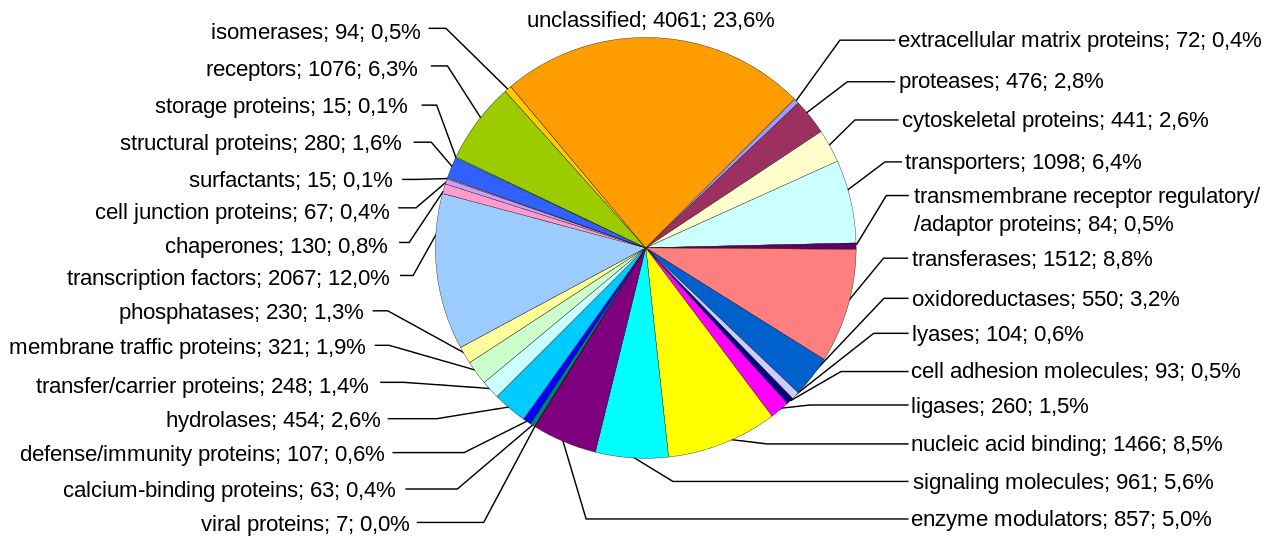
\includegraphics[width=0.50\textwidth]
		{pics/gbr2_1.png}
	\caption{Ada 23,6\% dari keseluruhan fungsi gen yang belum diketahui, sehingga pengetahuan tentang fungsi gen masih belum lengkap. \citep{haggstrom2014diagram}}
	\label{fig:gbr2.1}
\end{figure}

Data ekspresi gen yang masih mentah didapatkan dari percobaan di laboratorium menggunakan alat yang dinamakan dengan alat Genchip microarray. Data tersebut kemudian dilakukan pemrosesan awal untuk mendapatkan sebuah matriks ekspresi gen. Matriks ini memiliki data kolom dan baris, dimana kolom berisi data eksperimen, dan baris berisi nilai ekspresi pada tiap-tiap gen (\pic~\ref{fig:gbr2.3}) \citep{babu2004introduction}.

\begin{figure}
	\centering
	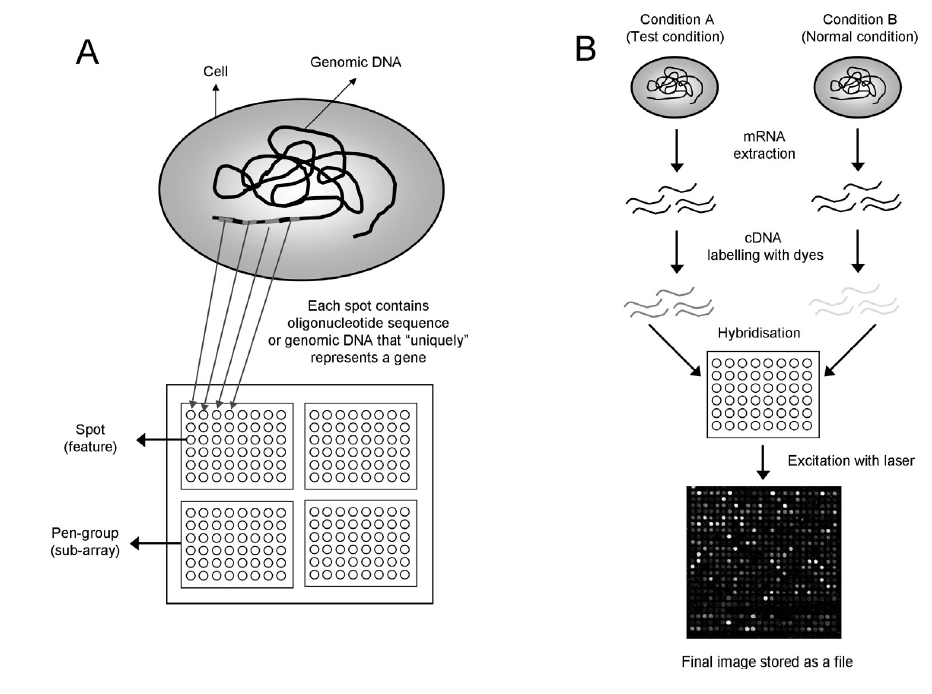
\includegraphics[width=0.95\textwidth]
		{pics/gbr2_2.png}
	\caption{Proses Keseluruhan Percobaan Microarray.\citep{yoon2006building}}
	\label{fig:gbr2.2}
\end{figure}

Pengukuran microarray direspresentasikan dengan tabel gen ekspresi, dimana bagian barisnya adalah fitur ekspresi gen, dan bagian kolom merepresentasikan pasien.

\begin{figure}
	\centering
	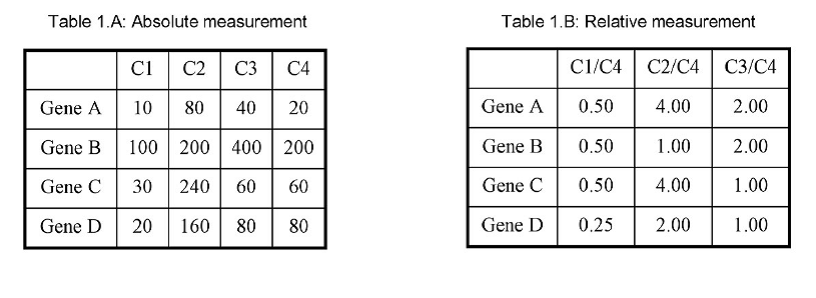
\includegraphics[width=0.95\textwidth]
		{pics/msr.png}
	\caption{Contoh data pengukuran percobaan microarray \citep{yoon2006building}}
	\label{fig:gbr2.3}
\end{figure}

Karena data microarray yang didapatkan dapat mencapai ribuan ekspresi dalam satu waktu secara simultan, maka data ini dapat sangat membantu dalam mengidentifikasi penyakit. Akan tetapi, hasil yang didapat dengan menganalisa beberapa data microarray yang dilakukan oleh dua percobaan yang berbeda tetapi dengan tujuan yang sama, dapat menghasilkan hasil yang sangat berbeda. Salah satu alasannya adalah terbatasnya sampel dan terlalu banyaknya profil ekspresi gen. Sehingga diperlukan metode testing statistik untuk memastikan bahwa data microarray tersebut memiliki tingkat signifikansi yang cukup, dan dipastikan bahwa perbedaan tersebut memang karena eksperimen, bukan karena kerusakan alat atau kesalahan prosedur eksperimen.
\begin{figure}
	\centering
	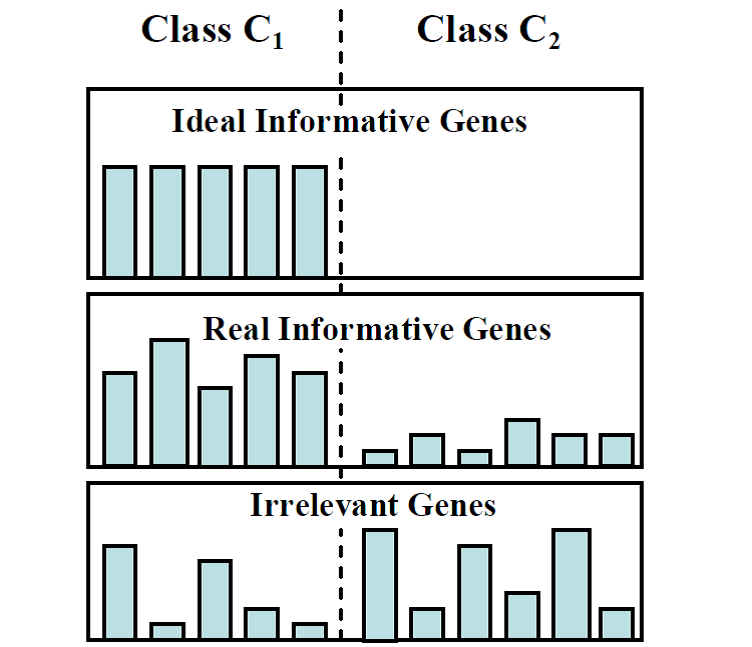
\includegraphics[width=0.8\textwidth]
		{pics/relevansigen.png}
	\caption{Perbandingan Ekspresi gen yang relevan dan informatif dibandingkan dengan gen yang tidak relevan\citep{babu2004introduction}}
	\label{fig:relevansi}
\end{figure}


%-----------------------------------------------------------------------------%
\section{Pemrosesan Data Microarray}
%-----------------------------------------------------------------------------%
Data yang dihasilkan dari alat \textit{microarray} ini berupa citra yang perlu diproses lebih lanjut. Sebelum data ekspresi gen dapat dianalisa lebih lanjut, perlu dilakukan pemrosesan awal yang berupa (i) perbaikan background, (ii) normalisasi data dan kemudian (iii) penyaringan data (iv) imputasi nilai yang hilang dan (v) seleksi fitur.
\begin{enumerate}
\item{\textbf{Perbaikan Background}}\\
Perbiakan background ini ditujukan untuk menghilangkan titik-titik \textit{noise} yang tidak berasal dari proses hibridisasi. Metode untuk perbaikan background ini adalah salah satu teknik yang banyak diajukan dalam penelitian\citep{fakoorusing}. 
\item{\textbf{Normalisasi}}\\
Tujuan dari normalisasi adalah untuk mengatur bias yang dihasilkan oleh variasi proses percobaan microarray. Metode normalisasi data microarray ada banyak, dan pada penelitian ini akan digunakan normalisasi standar untuk data microarray.
\item{\textbf{Penyaringan data}}
Tidak semua data yang didapat dari percobaan microarray bagus, kadangkala terjadi kesalahan alat dan noise yang diakibatkan oleh alat, oleh karena itu perlu disaring, mana data yang disebabkan oleh proses biologi, dan mana yang disebabkan oleh noise alat.
\item{\textbf{Imputasi Nilai yang Hilang}}\\
Tidak semua data ekspresi gen dapat kita dapatkan, dikarenakan rumitnya percobaan \textit{microarray}, kadangkala data tidak kita dapatkan, oleh sebab itu diperlukan metode untuk melakukan pendekatan statistik dalam memberikan perkiraan isi data dalam titik data yang hilang tersebut.
\item{\textbf{Seleksi Fitur}}\\
Setelah proses diatas, diperlukan teknik untuk menseleksi fitur pada data microarray. Ada banyak metode yang sudah diusulkan oleh para peneliti. Seperti pada tabel \ref{tabel1} dibawah. Dan pada titik inilah penelitian ini dijalankan.
\end{enumerate}

%-----------------------------------------------------------------------------%
\section{Ekstraksi Fitur dan Seleksi Fitur Pada Penelitian Sebelumnya}
%-----------------------------------------------------------------------------%
Pada tabel dibawah ditunjukkan perbandingan penelitian-penelitian ekstraksi fitur dengan menggunakan berbagai macam metode. Pada penelitian-penelitian sebelumnya, kebanyakan menggunakan metode statistik dan pembelajaran mesin yang dilakukan adalah \textit{supervised}, yaitu memiliki target. Seperti yang dilakukan oleh \citep{aliferis2003machine}, \cite{ramaswamy2001multiclass}. Sedangkan percobaan \textit{microarray} yang memiliki target, memiliki kelemahan, yaitu tidak semua target fitur gen diketahui kegunaannya. Oleh karena itu pendekatan \textit{unsupervised} dianggap lebih cocok untuk permasalahan seleksi fitur data \textit{microarray} \citep{haggstrom2014diagram}.
% Please add the following required packages to your document preamble:
% \usepackage{booktabs}
% \usepackage[normalem]{ulem}
% \useunder{\uline}{\ul}{}
\begin{table}
\centering
\caption{Perbandingan Metode Seleksi fitur  pada dataset microarray}
\label{tabel1}
\begin{tabular}{@{}llll@{}}
\toprule
Pengarang                                                            & Judul Paper                                                                                                                                                                     & Metode                                                                                                                            & Dataset                                                           \\ \midrule
\begin{tabular}[c]{@{}l@{}}C. Aliferis et al. \\ 2003\end{tabular}   & \begin{tabular}[c]{@{}l@{}}Machine learning models \\ for classication  of lung \\ cancer and selection of \\ genomic markers using \\ array gene expression data.\end{tabular} & \begin{tabular}[c]{@{}l@{}}Reduksi fitur secara rekursif \\ dan melakukan filter secara \\ asosiasi univariate\end{tabular}       & \begin{tabular}[c]{@{}l@{}}Lung Cancer \\ Microarray\end{tabular} \\
\begin{tabular}[c]{@{}l@{}}Ramaswamy, S. \\ et al. 2001\end{tabular} & \begin{tabular}[c]{@{}l@{}}Multiclass cancer diagnosis \\ using tumor gene expression \\ signatures.\end{tabular}                                                               & \begin{tabular}[c]{@{}l@{}}Pengurangan fitur secara \\ rekursif dengan \\ mengguanakan SVM\end{tabular}                           & \begin{tabular}[c]{@{}l@{}}Various \\ Microarray\end{tabular}     \\
\begin{tabular}[c]{@{}l@{}}Wang et al., \\ 2005\end{tabular}         & \begin{tabular}[c]{@{}l@{}}Gene-expression proles to \\ predict distant  metastasis \\ of lymph-node-negative \\ primary breast cancer.\end{tabular}                            & \begin{tabular}[c]{@{}l@{}}Mengkombinasikan seleksi \\ fitur yang  berbasis korelasi \\ dengan pendekatan assosiasi.\end{tabular} & \begin{tabular}[c]{@{}l@{}}Various \\ Microarray\end{tabular}     \\
\begin{tabular}[c]{@{}l@{}}Sharma et. Al, \\ 2012\end{tabular}       & \begin{tabular}[c]{@{}l@{}}Combining multiple \\ approaches for gene \\ microarray classification.\end{tabular}                                                                 & \begin{tabular}[c]{@{}l@{}}Mengkombinasikan banyak\\   pendekatan ekstraksi fitur\end{tabular}                                    & \begin{tabular}[c]{@{}l@{}}Various \\ Microarray\end{tabular}     \\ \bottomrule
\end{tabular}
\end{table}


%-----------------------------------------------------------------------------%
\section{Deep Learning}
%-----------------------------------------------------------------------------%

Sebelum tahun 2006, melakukan training dalam arsitektur \textit{deep learning} selalu gagal. Percobaan untuk melakukan training dengan \textit{feedforward neural network} memiliki hasil yang lebih buruk dibandingkan dengan arsitektur yang dangkal, yaitu arsitektur dengan layer 1 atau maksimum 2 layer.\\
Akan tetapi tiga paper yang terbit pada 2006 secara revolusioner telah merubah hal tersebut. Sehingga setelah tahun 2006 penelitian tentang \textit{deep learning} menjadi lebih intensif sampai sekarang dengan segala variasi arsitekturnya. Salah satu variasi arsitektur \textit{deep learning} yang dipakai dalam thesis ini adalah \textit{arsitektur Deep Belief Network (DBN)}. Ketiga paper tersebut adalah  \cite{hinton2006fast}, \cite{bengio2007greedy} dan \cite{poultney2006efficient}.

Learning secara \textit{unsupervised} menggunakan \textit{pretraining} secara tiap layer yang disebut dengan \textit{greedy layer-wise training}, yaitu training dilakukan  satu layer pada tiap satu waktu. Training ini dilakukan secara berjenjang pada layer selanjutnya. Kemudian dilakukan \textit{supervised training} untuk melakukan \textit{tuning parameter}, yang dimulai dari parameter hasil pretraining yang dilakukan sebelumnya.\\
DBN menggunakan \textit{Restricted Boltzmann Machine (RBM)} sebagai bagian terkecil dari layernya, yang menggunakan learning secara unsupervised yang merepresentasikan tiap layer. Sejak 2006, banyak sekali paper-paper yang mulai melakukan eksplorasi tentang deep learning ini, sehingga sejak saat itu deep learning merupakan salah satu teknik \textit{machine learning} yang paling populer, bahkan sampai saat ini \citep{fakoorusing}.

\section{Energy-Based Model (EBM) Adalah Bentuk General dari Restricted Boltzman Machine (RBM)}

EBM mengaitkan sebuah energi skalar pada setiap konfigurasi variable yang diinginkan. Proses learning bertujuan untuk memodifikasi fungsi energi sehingga bentuknya memiliki  sifat yang diinginkan. Sebagai contoh, misalnya diinginkan sebuah bentuk konfigurasi yang memiliki energi yang rendah, maka model probabilistik dari EBM didifinisikan sebagi distribusi probabilitas melalui fungsi energi sebagi berikut: \citep{poultney2006efficient}
\begin{equation}
p(x) = \frac {e^{-E(x)}} {Z}.
\end{equation}

Z adalah faktor normalisasi yang disebut sebagai fungsi partisi untuk menganalogikan dengan sistem fisika.
\begin{equation}
Z = \sum_x e^{-E(x)}
\end{equation}


EBM bisa dilatih dengan cara melakukan (stochastic) gradient descent pada negative log-likelihood (NLL)-nya secara empiris pada data training. Adapun untuk logistic regression akan didifinisikan terlebih dahulu log-likelihood $\mathcal{L}(\theta, \mathcal{D})$ dan fungsi loss-nya sebagai NLL $\ell (\theta, \mathcal{D})$ sebagai berikut:
\begin{equation}
\begin{aligned}
\mathcal{L}(\theta, \mathcal{D}) &= \frac{1}{N} \sum_{x^{(i)} \in
\mathcal{D}} \log\ p(x^{(i)}) \\
\ell (\theta, \mathcal{D}) &= - \mathcal{L} (\theta, \mathcal{D})
\end{aligned}
\end{equation}


Menggunakan stochastic gradient $-\frac{\partial  \log p(x^{(i)})}{\partial
\theta}$, dimana $\theta$ adalah parameter dari modelnya\citep{poultney2006efficient}.

\subsection{EBM dengan Hidden Units}

Pada banyak kasus, sampel $x$ biasanya tidak terobservasi secara penuh, atau akan ditambahkan variabel yang tidak terobservasi secara langsung yang disebut dengan hidden unit, dimana hal ini berguna untuk meningkatkan ekspresivitas dari model. Sehingga dikenalkan bagian yang terobservasi disini dilambangkan dengan $x$, dan sebuah bagian yang tersembunyi dilambangkan dengan $h$. Sehingga bisa ditulis sebagai:
\begin{equation}
P(x) = \sum_h P(x,h) = \sum_h \frac{e^{-E(x,h)}}{Z}.
\end{equation}

Pada kasus ini, untuk melakukan pemetaan rumus yang mirip dengan rumus 2.4 , akan dikenalkan notasi (yang merupakan inspirasi dari fisika) yaitu free energy $\mathcal{F}(x)$, yang didifinisikan sebagai berikut:

\begin{equation}
\mathcal{F}(x) = - \log \sum_h e^{-E(x,h)}
\end{equation}

Sehingga bisa diturunkan sebagai :
\[P(x) = \frac{e^{-\mathcal{F}(x)}}{Z} \text{ dengan } Z=\sum_x e^{-\mathcal{F}(x)}.\]

Data dari gradien NLL kemudian memiliki bentuk yang menarik yaitu:
\begin{equation}
- \frac{\partial  \log p(x)}{\partial \theta}
 = \frac{\partial \mathcal{F}(x)}{\partial \theta} -
       \sum_{\tilde{x}} p(\tilde{x}) \
           \frac{\partial \mathcal{F}(\tilde{x})}{\partial \theta}.
\end{equation}

Gradien diatas memiliki dua istilah, dimana hal tersebut mereferensikan pada fase positif dan fase negatif. Istilah positif dan negatif ini tidak merujuk pada tanda (positif/negatif)  persamaan, akan tetapi merefleksikan efek pada kepadatan probabilitas yang didefinisikan oleh model. Istilah pertama, menambah probabilitas data training (dengan cara mengurangi free energy yg berhubungan), sedangkan istilah kedua mengurangi probabilitias sampel yang digenerasi oleh model \citep{poultney2006efficient}.\\

Biasanya sulit untuk menentukan gradien secara analitis, oleh karena berhubungan dengan komputasi dari $E_P [ \frac{\partial \mathcal{F}(x)} {\partial \theta} ]$. Dikarenakan hal ini merupakan ekspektasi semua kemungkinan konfigurasi input $x$ (pada distribusi $P$ yang dibentuk oleh model).\\
Oleh karena itu, langkah pertama agar bisa dikomputasi secara analitis maka dilakukan estimasi ekspektasi menggunakan jumlah yang pasti dari sampel pada model. Sampel digunakan untuk mengestimasi gradien dari fase negatif yang direferensikan sebagai partikel negatif, dimana disimbolkan sebagai $\mathcal{N}$. Kemudian, gradien bisa ditulis sebagai \citep{poultney2006efficient} : 

\begin{equation}
- \frac{\partial \log p(x)}{\partial \theta}
 \approx
  \frac{\partial \mathcal{F}(x)}{\partial \theta} -
   \frac{1}{|\mathcal{N}|}\sum_{\tilde{x} \in \mathcal{N}} \
   \frac{\partial \mathcal{F}(\tilde{x})}{\partial \theta}.
\end{equation}
Dimana secara ideal, elemen seperti $\tilde{x}$ dari $\mathcal{N}$ disampel menurut $P$ (sebagai contoh adalah menggunakan teknik sampling Monte-Carlo). Dengan rumus diatas, secara praktis hampir bisa melakukan algoritma stochastic, hanya saja partikel negatif $\mathcal{N}$ belum bisa diekstraksi. Oleh karena itu, pada literatur dengan metode Markov Chain Monte Carlo, sangat bagus digunakan pada model Restricted Boltzmann Machine (RBM) yang merupakan bentuk spesifik dari model EBM \citep{tutorial2014lisa}.


%-----------------------------------------------------------------------------%
\section{Restricted Boltzmann Machine}
%-----------------------------------------------------------------------------%
Boltzmann Machines (BMs) adalah bentuk khusus dari log-linear Markov Random Field (MRF), dengan kata lain, dimana fungsi energi adalah linear pada parameter bebasnya. Agar membuat BM cukup bisa merepresentasikan distribusi yang kompleks(dengan kata lain, berangkat dari setting parameter yang terbatas kepada non paramter), diasumsikan bahwa beberapa variabel tidak terobserbasi sehingga disebut hidden. Dengan memiliki variabel hidden, bisa dilakukan peningkatan kapasitas model dari BM. RBM, selanjutnya membuat BM yang terbatas pada variabel tanpa koneksi visibel-visibel dan hidden-hidden. Seperti pada gambar \ref{fig:rbm} \citep{hinton2006fast}\\
\begin{figure}
	\centering
	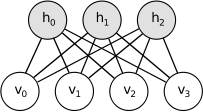
\includegraphics[width=0.3\textwidth]
		{pics/rbm.png}
	\caption{Grafik yang Menggambarkan RBM}
	\label{fig:rbm}
\end{figure}

Fungsi energi $E(v,h)$ pada RBM didefinisikan sebagai persamaan \ref{eq:rbm1}.

\begin{equation}
E(v,h) = - b'v - c'h - h'Wv
\label{eq:rbm1}
\end{equation}

Dimana $W$ merepresentasikan bobot yang terkoneksi antara unit hidden dan visible dan $b$, $c$ adalah bias dari visible dan hidden secara berurutan.\\

Hal ini bisa diterjemahkan dalam bentuk persamaan energi bebas $\mathcal{F}(v)$ seperti dibawah:
\[\mathcal{F}(v)= - b'v - \sum_i \log \sum_{h_i} e^{h_i (c_i + W_i v)}.\]
Dikarenakan struktur RBM yang spesifik, visibel dan hidden adalah independen secara bersyarat antara satu dengan lainnya. Dengan menggunakan sifat tersebut, maka dapat dituliskan :

\[p(h|v) = \prod_i p(h_i|v)\]
\[p(v|h) = \prod_j p(v_j|h).\]

\subsection{RBMs yang Menggunakan Unit Biner}

Kasus umum jika menggunakan unit biner (dimana $v_j$ dan $h_i \in
\{0,1\})$, yang didapat dari persamaan (6) dan (2), versi probabilistik dari fungsi aktivasi neuron adalah sebagai berikut\citep{hinton2006reducing}:

\begin{equation}
P(h_i=1|v) = sigm(c_i + W_i v)
\end{equation}

\begin{equation}
P(v_j=1|h) = sigm(b_j + W'_j h)
\end{equation}

Selanjutnya, energi bebas dari RBM dengan unit biner, disederhanakan menjadi persamaan:

\begin{equation}
\mathcal{F}(v)= - b'v - \sum_i \log(1 + e^{(c_i + W_i v)}).
\end{equation}

\subsection{Update Persamaan dengan Unit Biner}

Menghubungkan persamaan (5) dengan (9), didapatkan gradien log-likelihood untuk RBM dengan unit biner sebagai berikut:

\begin{equation}
\begin{aligned}
- \frac{\partial{ \log p(v)}}{\partial W_{ij}} &=
    E_v[p(h_i|v) \cdot v_j]
    - v^{(i)}_j \cdot sigm(W_i \cdot v^{(i)} + c_i) \\
-\frac{\partial{ \log p(v)}}{\partial c_i} &=
    E_v[p(h_i|v)] - sigm(W_i \cdot v^{(i)})\\
-\frac{\partial{ \log p(v)}}{\partial b_j} &=
    E_v[p(v_j|h)] - v^{(i)}_j
\end{aligned}
\label{eq:eq2.10}
\end{equation}

\section{Sampling pada RBM}

Sampel dari $p(x)$ bisa didapat dengan menjalankan Markov chain sampai konvergen dengan menggunakan gibbs samping sebagai operator transisi. \\

Gibbs sampling dari join variable random sebanyak $N$ dari $S=(S_1, ... , S_N)$ merupakan urutan sebanyak $N$ sampling dari sub-steps dalam bentuk $S_i \sim p(S_i | S_{-i})$ dimana $S_{-i}$ berisi $N-1$ variabel random lain didalam $S$ tetapi diluar $S_i$.

Untuk RBM, $S$ berisi himpunan dari visible dan hidden unitnya. Akan tetapi, dikarenakan unit ini dipenden secara kondisional, maka salah satunya bisa dilakukan gibbs sampling. Pada setting disini, unit visible disampel secara simultan given nilai fix dari hidden unitnya. Demikian sebaliknya, hidden unitnya disampel secara simultan given unit visibelnya.Sehingga satu langkah Markov chain adalah sebagai berikut: 

\[h^{(n+1)} \sim sigm(W'v^{(n)} + c)\] 
\[v^{(n+1)} \sim sigm(W h^{(n+1)} + b),\]

Dimana $h^{(n)}$ menunjik pada himpunan semua hidden unit pada nilai yang ke-$n$ langkah dari Markov chain. Yang artinya adalah sebagai contoh, $h^{(n+1)}_i$ adalah secara random dipilih antara 1 (versus 0) dengan nilai probabilitas $sigm(W_i'v^{(n)} + c_i)$, demikian juga, $v^{(n+1)}_j$ adalah dipilih secara random antara 1 (versus 0) dengan probabilitas $sigm(W_{.j} h^{(n+1)} + b_j)$.

Hal ini seperti digambarkan pada gambar \ref{fig:markov_chain}
\begin{figure}
	\centering
	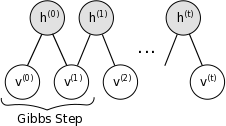
\includegraphics[width=0.3\textwidth]
		{pics/markov_chain.png}
	\caption{Gibbs Sampling}
	\label{fig:markov_chain}
\end{figure}


Oleh karena $t \rightarrow \infty$, maka sampel $(v^{(t)}, h^{(t)})$ bisa dipastikan akan akurat dalam mensampel $p(v,h)$.

Secara teori, tiap parameter diupdate pada proses learning dibutuhkan satu rantai tersebut untuk konvergen. Akan tetapi hal ini sangat mahal komputasinya. Sehingga banyak diajukan algoritma untuk melatih RBM agar sampel $p(v,h)$ efisien, disaat proses learningnya.

\section{Contrastive Divergence (CD-k)}

Contrastive Divergence(CD) menggunakan trik untuk mempercepat proses sampling: Dikarenakan yang diinginkan adalah $p(v) \approx p_{train}(v)$ (distribusi data yang asli), initialisasi  Markov chain dengan contoh data training (dimana, berasal dari distribusi yang mendekati $p$, pada distribusi final dari $p$). CD tidak menunggu rantai untuk konvergen. Sampel didapatkan setalah langkah ke-$k$ dari Gibbs sampling. Pada prakteknya, $k=1$ sudah menghasilkan hasil yang baik.\\

\section{Persistent CD}

Persistent CD (P-CD) [Tieleman08] menggunakan pendekatan lain untuk mensampling $p(v,h)$. Hal ini bergantung hanya pada Markov chain tunggal, yang memiliki kondisi yang persisten (dimana, tidak melakukan restart chain pada setiap sampel yang terobservasi). Pada setiap umpdate parameter, akan di ekstraksi sampel baru dengan penjalankan chain pada langkah ke-$k$. Kondisi chain akan dipertahankan pada update selanjutnya.\\
Intuisinya adalah jika update parameternya cukup kecil dibaningkan dengan rate campuran dari Markov Chain, maka hal ini bisa mengejar perubahan modelnya.



%-----------------------------------------------------------------------------%
\section{Deep Belief Network}
%-----------------------------------------------------------------------------%

\cite{hinton2006fast} menunjukkan bahwa RBM bisa dijajar dan dilatih secara greedy untuk membentuk sebuah jaringan yang dinamakan dengan \textit{Deep Belief Network (DBN)}. DBN adalah model grafis dimana bisa melakukan learning untuk mengekstraksi representasi hirarki yang mendalam (deep) dari data training. Hal ini memodelkan distribusi gabungan antara vektor $x$ sebagai observer dan $\ell$ layer hidden $h^k$ sebagai berikut:

\begin{equation}
P(x, h^1, \ldots, h^{\ell}) = \left(\prod_{k=0}^{\ell-2} P(h^k|h^{k+1})\right) P(h^{\ell-1},h^{\ell})
\end{equation}

Dimana $x=h^0, P(h^{k-1} | h^k)$ adalah distribusi kondisional untuk unit visible dikondisikan pada unit hidden pada level $k$ dan  $P(h^{\ell-1}, h^{\ell})$ adalah distribusi gabungan visible-hidden pada level teratas dar RBM. Seperti diilustrasikan pada gambar \ref{fig:dbn3}.

\begin{figure}
	\centering
	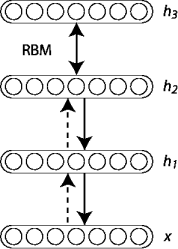
\includegraphics[width=0.3\textwidth]
		{pics/DBN3.png}
	\caption{Arsitektur Deep Belief Network (DBN) yang merupakan gabungan dari RBM yang dibuat bertingkat}
	\label{fig:dbn3}
\end{figure}


Prinsip dari \textit{greedy layer-wise unsupervised training} bisa di aplikasikan pada DBN dengan RBM sebagai bagian pada tiap layernya [hinton] [bengio]. Pada prinsipnya prosesnya adalah sebagai berikut:
\begin{enumerate}
\item Latih layer pertama ssebagai RBM yang memodelkan input $x = h^{(0)}$ sebagai visible layernya.
\item Gunakan layer pertama untuk mendapatkan representasi input yang digunakan sebagai data untuk layer kedua. Ada dua solusi yang sama. Representasi ini bisa dipilih sebagai rata-rata dari aktivasi $p(h^{(1)}=1|h^{(0)})$ atau sampel dari $p(h^{(1)}|h^{(0)})$.
\item Train layer kedua sebagai RBM dengan mengambil data transformasi (sampel atau rata-rata aktivasi) sebagai training (untuk layer visible dari RBM tersebut).
\item Iterasikan (2 dan 3) untuk semua layer yang diinginkan, setiap waktu dengan mempropagasikan keatas antara sampel atau nilai rata-ratanya.
\item Fine-tune semua parameter dari arsitektur dengan log-likelihood DBN atau dengan kriteria secara supervised setelah menambahkan layer supervised untuk memprediksikan kelas, sebagai contoh misalnya layer logistic regression.
\end{enumerate}

Pada kasus ini, akan difokuskan pada fine-tuning dengan melakukan gradien descent menggunakan klassifier logistic regression dimana digunakan untuk mengklasifikasikan input x berdasar pada output dari hidden layer $h^{(l)}$ dari DBN. Fine-tune kemudian dilakukan melalui gradien descent dari NLL fungsi costnya. Dikarenakan gradien secara supervised adalah hanya non-null untuk bobot dan bias pada hidden layer pada tiap-tiap layer, maka prosedur ini serupa dengan menerapkan initialisasi parameter dari arsitektur MLP yang deep dengan bobot dan bias dari hidden layer yang didapat pada proses training unsupervised diatas.

\section{Cost}
Cost merupakan variabel yang menggambarkan \textit{Negative Log Likelihood}. Yang memiliki bentuk persamaan sebagai berikut:
\begin{equation}
\frac{1}{|\mathcal{D}|} \mathcal{L} (\theta=\{W,b\}, \mathcal{D}) =
            \frac{1}{|\mathcal{D}|} \sum_{i=0}^{|\mathcal{D}|}
                \log(P(Y=y^{(i)}|x^{(i)}, W,b)) \\
            \ell (\theta=\{W,b\}, \mathcal{D})
\end{equation}

Dalam kode python dituliskan:
\begin{center}
cost = classifier.negative\_log\_likelihood(y)
\end{center}

Semakin kecil cost, menunjukkan semakin kecil error rekonstruksinya. Hal ini menunjukkan bahwa, data rekonstruksi mendekati bentuk data konstruksinya (diambil dari data training).


\section{Training Secara Greedy Layer-Wise}

Algoritma training deep learning secara greedy layer-wise terbukti bisa bekerja dengan baik, sebagai contoh 2 layer DBN dengan hidden layer $h^{(1)}$ dan $h^{(2)}$ dengan parameter bobot berurutan adalah $W^{(1)}$ dan $W^{(2)}$, \citep{hinton2006reducing} maka $\log
p(x)$ bisa ditulis sebagai:
\begin{equation}
\begin{aligned}
\log p(x) = &KL(Q(h^{(1)}|x)||p(h^{(1)}|x)) + H_{Q(h^{(1)}|x)} + \\
            &\sum_h Q(h^{(1)}|x)(\log p(h^{(1)}) + \log p(x|h^{(1)})).
\end{aligned}
\label{eq:equ2}
\end{equation}

$KL(Q(h^{(1)}|x) || p(h^{(1)}|x))$ merepresentasikan KL divergence antara posterior $Q(h^{(1)}|x)$ dari RBM pertama jika hal ini sendirian, dan probabilitas $p(h^{(1)}|x)$ untuk layer sayng sama tapi didifinisikan oleh keseluruhan DBN (sebagai contoh, perhitungan prior $p(h^{(1)},h^{(2)}$) didefinisikan sebagai top-level RBM). $H_{Q(h^{(1)}|x)}$ adalah entropy dari distribusi $Q(h^{(1)}|x)$.\\
Hal ini bisa ditunjukkan bahwa jika diinitialisasi kedua layer hidden sehingga $W^{(2)}={W^{(1)}}^T, Q(h^{(1)}|x)=p(h^{(1)}|x)$ dan KL divergence nya adalah null. Maka jika di lakukan learning pada level awal RBM dan kemudian parameter $ W^{(1)}$ dibuat tetap, kemudian dilakukan optimasi pada persamaan \ref{eq:equ2} terhadap $W^{(2)}$ bisa meningkatkan likelihood dari $p(x)$.
Jika diisolasi hanya pada $W^{(2)}$ sehinggi didapatkan:

\[\sum_h Q(h^{(1)}|x)p(h^{(1)})\]

Melakukan optimasi persamaan ini dengan memperhatikan jumlah $W^{(2)}$ training pada tingkat RBM selanjutnya, menggunakan output dari $Q(h^{(1)}|x)$ sebagai distribusi training untuk RBM yang pertama.

%-----------------------------------------------------------------------------%
\section{Logistic Regression}
%-----------------------------------------------------------------------------%
\textit{Logistic Regression} adalah salah satu klassifier yang paling dasar pembentuk dari MLP. Penjelasannya akan dimulai dari bentuk model dasarnya serta notasi matematisnya.

\subsection{Model Logistic Regression}
\textit{Logistic regression} adalah klasifier yang linear dan probabilistik. Diparameterkan dengan matrik bobot $W$ dan vektor bias $b$. Proses klasifikasinya adalah dengan cara memproyeksikan vektor input kedalam himpunan \textit{hyperplane}, dimana berkorespondensi pada kelasnya. Jarak dari input ke \textit{hyperplane} merefleksikan probabilatas dari input adalah berkorespondensi dari anggota kelasnya.\\
Secara matematis, probabilitas vektor input $x$ adalah anggota dari kelas $i$, isi dari variabel \textit{stochastic} $Y$, bisa ditulis sebagai berikut:
\begin{equation}
\begin{aligned}
P(Y=i|x, W,b) &= softmax_i(W x + b) \\
              &= \frac {e^{W_i x + b_i}} {\sum_j e^{W_j x + b_j}}
\end{aligned}
\end{equation}

Prediksi dari model berupa $y_{pred}$ adalah kelas dimana probabilitasnya maksimal, secara spesifik ditulis sebagai:
\begin{equation}
y_{pred} = {\rm argmax}_i P(Y=i|x,W,b)
\end{equation}

\subsection{Mendefinisikan Lost Function dari Logistic Regression}
Melakukang \textit{learning} pamameter model dengan cara meminimalisasi \textit{Lost Function}. Pada kasus \textit{logistic regression} yang multi-kelas, sangat umum digunakan minimisasi \textit{negative log likelihood (NLL)} yang ekivalen dengan memaksimalkan likelihood dari data set $\cal{D}$ pada model yang diparameterkan oleh $\theta$. Definisi dari likelihood $\cal{L}$ dan loss $\ell$ maka:
\begin{equation}
\begin{aligned}
\mathcal{L} (\theta=\{W,b\}, \mathcal{D}) =
  \sum_{i=0}^{|\mathcal{D}|} \log(P(Y=y^{(i)}|x^{(i)}, W,b)) \\
\ell (\theta=\{W,b\}, \mathcal{D}) = - \mathcal{L} (\theta=\{W,b\}, \mathcal{D})
\end{aligned}
\end{equation}
Untuk meminimisasi, digunakan \textit{stochastic gradient descen with minibatches (MSGD)} \citep{hinton2006fast}.


%-----------------------------------------------------------------------------%
\section{Multi Layer Perceptron}
%-----------------------------------------------------------------------------%

Arsitektur selanjutnya yang akan dibahas adalah \textit{Multi Layer Perceptron (MLP)} Arsitektur MLP ini bisa dilihat sebagai klasifier \textit{Logistic Regression} dimana input pada awalnya ditransformasikan menggunakan transformasi non linear $\Phi$. Transformasi ini memproyeksikan data input kepada \textit{space} dimana hal ini bisa terseparasi secara linear. Layer tengah ini direferensikan sebagai \textit{hidden layer}. Satu hidden layer sebenarnya sudah cukup untuk membuat MLP sebagai aproksimator universal. Akan tetapi, ada banyak keuntungan untuk menggunakan hidden unit yang lebih dari satu layer, hal inilah yang digunakan sebagai konsep dasar dari deep learning. Algoritma untuk melakukan \textit{training} dari MLP yang paling sering dipakai adalah algoritma \textit{back-propagation} \citep{tutorial2014lisa}.

\subsection{Model MLP}

MLP atau sering disebut juga dengan Artificial Neural Network (ANN) adalah Perceptron yang dibentuk menjadi sebuah jaringan. MLP dengan layer tunggal bisa direpresentasikan secara grafis seperti pada  \pic~\ref{fig:mlp} berikut.

\begin{figure}
	\centering
	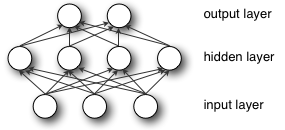
\includegraphics[width=0.45\textwidth]
		{pics/mlp.png}
	\caption{Arsitektur Layer Tunggal MLP}
	\label{fig:mlp}
\end{figure}

Secara formal, hidden layer tunggal dari MLP adalah sebuah fungsi $f: R^D \rightarrow R^L$, dimana $D$ aadlah ukuran dari vektor input $x$ dan $L$ adalah ukuran dari output vektor $f(x)$ sehingga dengan menggunakan notasi matriks sebagai berikut :

\begin{equation}
f(x) = G( b^{(2)} + W^{(2)}( s( b^{(1)} + W^{(1)} x))),
\end{equation}

Dengan vektor bias $b^{(1)}, b^{(2)}$; dan matrik bobot $W^{(1)}, W^{(2)}$ dan fungsi aktivasinya adalah $G$ dan $s$. Sedangkan vektor $h(x) = \Phi(x) = s(b^{(1)} + W^{(1)} x)$ merupakan \textit{hidden layer}. Setiap kolom $W^{(1)}_{\cdot i}$ merepresentasikan bobot dari unit input yang ke-$i$ dari \textit{hidden unit}. Pilihan fungsi aktifasinya bisa menggunakan tanh, atau fungsi sigmoid.
\begin{equation}
\begin{aligned}
tanh(a)&= \frac{(e^a-e^{-a})}{(e^a+e^{-a})} \\
sigm(a)&=\frac{1}{(1+e^{-a})}
\end{aligned}
\end{equation}
Kedua fungsi aktivasi yaitu tanh dan sigmoid adalah fungsi skalar ke skalar akan tetapi bisa diekstensikan menjadi vektor atau tensor yang diaplikasikan secara \textit{element wise}.\\
Vektor output didapatkan dengan: $o(x) = G(b^{(2)} + W^{(2)} h(x))$. Probabilitas dari keanggotaan kelas didapat dari memilih G sebagai fungsi \textit{softmax} (untuk kasus klasifikasi multi-kelas).\\
Untuk melakukan \textit{training} MLP dilakukan \textit{learning} parameter dari model menggunakan \textit{Stochastic Gradien Descent} dengan dibagi menjadi bagian kecil-kecil atau disebut dengan \textit{minibatch}. Himpunan parameter pembelajarkan ditulis sebagai himpungan $\theta = \{W^{(2)},b^{(2)},W^{(1)},b^{(1)}\}$. Mendapatkan gradien $\partial{\ell}/\partial{\theta}$ didapatkan dengan menerapkan algoritma \textit{backpropagation} \citep{tutorial2014lisa}

\section{Metode Bonferroni untuk Evaluasi}

Di dalam statistik, testing hipotesis adalah berdasar pada menolak hipotesa 0 apabila kebolehjadian data yang diobservasi dibawah hipotesa 0 adalah rendah. Jika dilakukan perbandingan berganda atau dilakukan pengetesan hipotesa, maka kemungkinan untuk terjadi sebuah peristiwa yang langka menjadi meningkat, oleh karena itu, kebolehjadian untuk menolak hipotesa 0 menjadi meningkat pula ( error tipe 1 meningkat ). Oleh karena itu dibutuhkan untuk sebuah metode koreksi untuk menjaga agar error tipe I nya bisa dikoreksi.

Metode koreksi Bonferroni adalah berbasis pada ide dimana jika eksperimen dilakukan untuk melakukan testing pada hipotesa sebanyak $m$, maka untuk memelihara \textit{familywise error rate (FWER)} adalah untuk melakukan testing hipotesis secara individu dengan level signifikansi $1/m$ dikalikan dengan level maksimum keseluruhan yang diinginkan.

Jika level signifikansi yang diinginkan semua anggota dari test adalah $\alpha$, maka koreksi bonferroni akan melakukan testing secara individual dengan level signifikansinya adalah $\alpha/m$. Sebagai contoh jika testing percobaan $m=8$ dengan hipotesa yang diinginkan $\alpha =0.05$ maka kereksi akan melakukan testing secara individual pada hipotesis pada $\alpha =0.05/8=0.00625$ \citep{hochberg1988sharper}

\subsection{Definisi}
Diberikan $H_{{1}},...,H_{{m}}$ adalah sebuah keluarga hipotesa dan $p_{{1}},...,p_{{m}}$ adalah secara berurutan merupakan \textit{p-value}-nya. FWER adalah probabilitas untuk menolak setidaknya satu dari $H_{{i}}$; sehingga setidaknya ada satu error tipe I. Maka koreksi bonferroni menyatakan bahwa menolak hipotesa null untuk semua $p_{{i}}\leq {\frac  {\alpha }{m}}$ yang mengontrol FWER. Dibuktikan dengan :
\begin{equation}
FWER = P\left\{ \bigcup_{i=1}^{m_0}\left(p_{i}\leq\frac{\alpha}{m}\right)\right\} \leq\sum_{i=1}^{m_0}\left\{P\left(p_{i}\leq\frac{\alpha}{m}\right)\right\}\leq m_{0}\frac{\alpha}{m}\leq m\frac{\alpha}{m}=\alpha
\end{equation}
Kontrol ini tidak memerlukan asumsi tentang ketergantungan antara p-value-nya \citep{hochberg1988sharper}.
%-----------------------------------------------------------------------------%
\chapter{\babTiga}
%-----------------------------------------------------------------------------%

Penelitian ini dibagi menjadi empat tahap: (1) Mendapatkan data microarray dan pengolahan awal; (2) Perancangan algoritma; (3) Melakukan eksperimen untuk mendapatkan \textit{hyperparameter} yang optimal. Kemudian dilanjutkan dengan  testing dan evaluasi. Gambaran umum dari penelitian ini seperti pada \pic~\ref{fig:overview}




%-----------------------------------------------------------------------------%
\section{Gambaran Umum Penelitian}
%-----------------------------------------------------------------------------%

Secara garis besar, penelitian ini dibagi menjadi beberapa tahapan. Yang pertama adalah tahapan persiapan yaitu mendapatkan data \textit{microarray} kemudian mengolahnya menjadi data yang siap untuk dilakukan proses seleksi fitur dan tahapan pelatihan \textit{deep learning}. Yaitu dengan membagi 80\% data untuk training, 15\% data untuk  validasi dan 5\% data untuk testing.\\
Bagian kedua adalah  membangun model DBN dengan teknik \textit{unsupervised learning}. Untuk mendapatkan model terbaik   secara \textit{greedy} pada tiap-tiap layer RBM-nya. Dimana dilakuan tuning \textit{hyperparameter} (jumlah kedalaman layer, jumlah \textit{hidden unit} pada tiap layernya) digunakan untuk mendapatkan struktur \textit{hyperparameter} yang cocok dengan ciri khas dari data \textit{microarray}. Oleh karena itu diperlukan banyak percobaan untuk mendapatkan hasil yang bagus. \\
Bagian ketiga, adalah \textit{supervised learning}, dimana merupakan  evaluasi sementara dari tahap yang kedua. Dibuat layer output berupa \textit{logistic regression}, yang digunakan untuk menguji sementara hasil dari proses \textit{pretraining} untuk mengklasifikasikan pasien kanker dan pasien normal menggunakan dataset validasi dan dataset testing. \\
Bagian keempat merupakan bagian yang terpenting karena  dimana ide thesis ini dibuat. Yaitu melakukan perankingan gen untuk mencari gen yang paling informatif yang didapatkan dari model pada percobaan sebelumnya. Dimana algoritma seleksi fitur untuk multi-step ranking dijalankan agar didapatkan \textit{biomarker}.\\

\begin{figure}
	\centering
	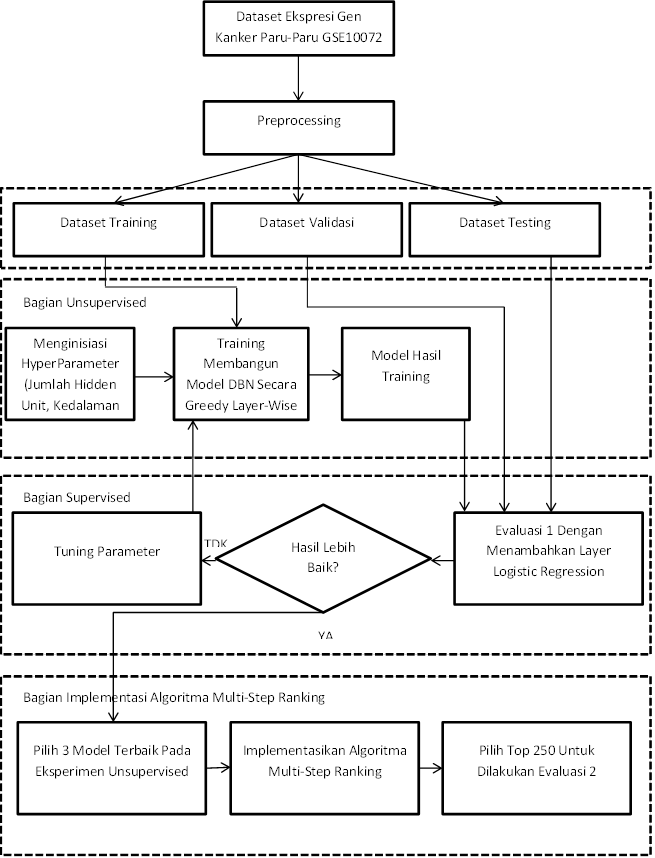
\includegraphics[width=0.9\textwidth]
		{pics/overview.png}
	\caption{Overview Penelitian}
	\label{fig:overview}
\end{figure}

Tahapan terakhir adalah tahap evaluasi akhir, yaitu  akan dilakukan dua kali evaluasi, yang pertama evaluasi  dengan cara membandingkan evaluasi 1 (\textit{logistic regression} sebelum dilakukan seleksi fitur) dengan evaluasi 2 (MLP setelah dilakukan seleksi fitur). Hasil dari kedua proses ini dibandingkan apakah terjadi perbaikan performa klasifikasinya. \\
\begin{figure}
	\centering
	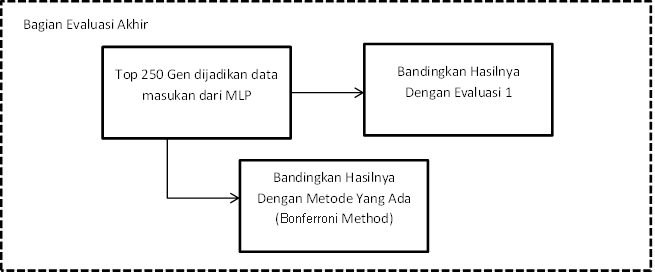
\includegraphics[width=0.9\textwidth]
		{pics/evaluasi2.png}
	\caption{Overview Metode Evaluasi}
	\label{fig:evaluasi2}
\end{figure}
Untuk evaluasi selanjutnya yaitu dilakukan konfirmasi, dimana hasil dari perankingan gen tersebut dibandingkan dengan penelitian tentang biomarker sebelumnya. Apakah gen biomarker yang ditemukan pada penelitian ini memiliki signifikansi dibandingkan dengan teknik sebelumnya.\\
\begin{figure}
	\centering
	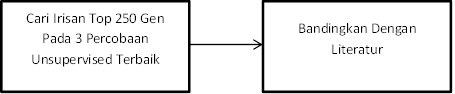
\includegraphics[width=0.8\textwidth]
		{pics/evaluasi3.png}
	\caption{Metode Untuk Mengkonfirmasi Biomarker}
	\label{fig:evaluasi2}
\end{figure}

%-----------------------------------------------------------------------------%
\section{Desain Metode Perangkingan Bobot Secara Multi Step Untuk Mendapatkan Gen Biomarker}
%-----------------------------------------------------------------------------
Pada penelitian ini, akan dibangun sebuah teknik pencarian \textit{Biomarker} dengan metode seleksi fitur gen. Metode ini menerapkan perankingan gen secara \textit{multi step} terhadap model yang didapatkan pada proses \textit{training} yang dilakukan secara \textit{unsupervised}. Arsitektur untuk mendapatkan modelnya adalah digunakan  arsitektur \textit{Deep Belief Network (DBN)} yang merupakan bagian dari metode \textit{deep learning}. Metode perankingan yang digunakan adalah modifikasi dari algoritma seleksi fitur untuk \textit{logistic regression} yang dilakukan oleh \cite{shevade2003simple}. Akan tetapi metode ini memiliki masalah dalam  mengeliminasi fitur jika diterapkan secara langsung pada model DBN, dikarenakan parameter bobot (W) dan bias (b) ditempatkan disetiap fitur dan model ini hanya memiliki satu layer dibandingkan dengan DBN yang memiliki banyak layer. \\
Pada DBN, \textit{hidden unit} yang paling sering aktif adalah \textit{hidden unit} yang lebih penting dibandingkan dengan unit yang jarang aktif, oleh karena itu \textit{hidden unit} ini memiliki parameter bobot yang lebih besar dibandingkan dengan \textit{hidden unit} yang jarang aktif pada saat proses \textit{training} dilakukan. Pemilihan fitur dilakukan dengan meranking unit-unit yang memiliki bobot tertinggi dimulai dari \textit{layer output} mundur secara multi-step menuju \textit{layer input} untuk mendapatkan fitur gen yang paling berpengaruh terhadap model. Kemudian dilakukan eliminasi bobot pada \textit{hidden unit} per layernya secara \textit{multi step}. Selanjutnya akan dipilih sebanyak \textit{top-n} gen dari hasil perankingan ini untuk dievaluasi apakah \textit{Biomarker} yang ditemukan tersebut informatif atau tidak. Seperti digambarkan pada bagan \pic~\ref{fig:multistep1} \\

\begin{figure}
	\centering
	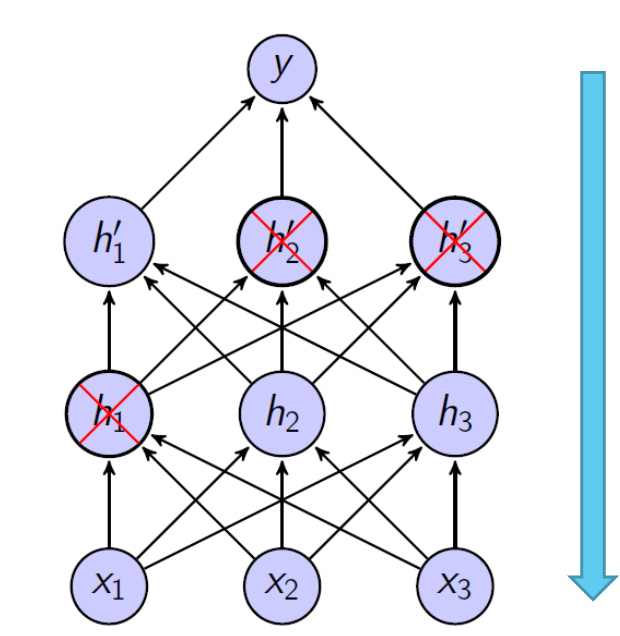
\includegraphics[width=0.3\textwidth]
		{pics/multistep1.png}
	\caption{Hidden unit yang paling sering aktif adalah neuron yang paling penting. Sedangkan yang Kurang Penting Dihapus dengan arah mundur Secara Multi-step \citep{duh2014deep}}
	\label{fig:multistep1}
\end{figure}

\subsection{Perhitungan Seleksi Fitur dengan Multi-Step Ranking }

Contoh dibawah adalah contoh penyederhanaan dari proses multi-step ranking yang diajukan. Pada prakteknya, \textit{visible unit} dan \textit{hidden unit} memiliki jumlah yang besar. Sebagai contoh, pada kasus data kanker paru-paru yang diteliti ini memiliki fitur 22 ribu gen yang di ukur secara simultan dalam satu percobaan.

\begin{figure}
	\centering
	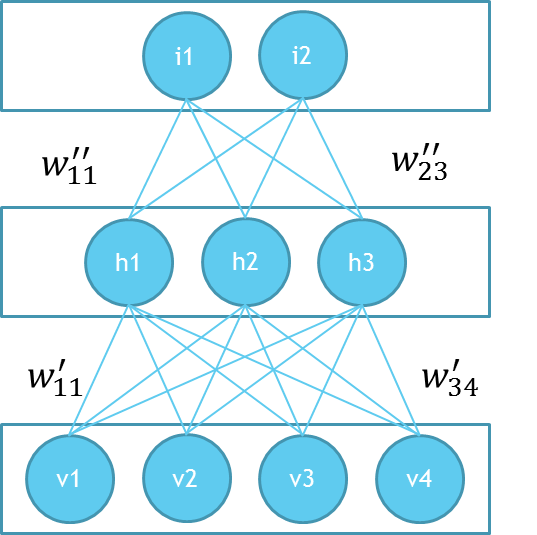
\includegraphics[width=0.95\textwidth]
		{pics/multistep2.png}
	\caption{Contoh Perhitungan tahap pertama dimulai dari top hidden unit }
	\label{fig:multistep2}
\end{figure}

\begin{figure}
	\centering
	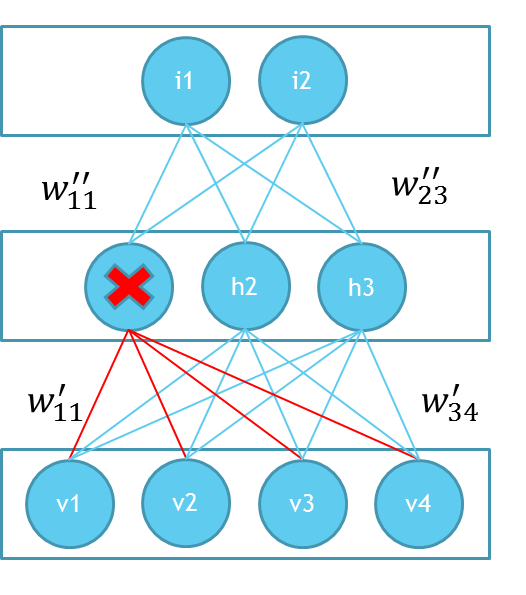
\includegraphics[width=0.95\textwidth]
		{pics/multistep3.png}
	\caption{Contoh Perhitungan tahap pertama dimulai dari top hidden unit }
	\label{fig:multistep3}
\end{figure}

Perhitungan diatas secara iteratif dilakukan mulai dari layer output mundur sampai layer input.

%-----------------------------------------------------------------------------%
\section{Implementasi Metode Perangkingan Bobot Secara Multi Step Untuk Mendapatkan Gen Biomarker}
%-----------------------------------------------------------------------------%
Implementasi multi-step ranking dengan menggunakan python:\\
Listing 3.4 : Implementasi Multi-Step Ranking di python
\lstinputlisting[language=python, frame=single, basicstyle=\tiny]{snip/multistep_rank.py}

Contoh implementasi multistep rank pada model yang disimpan pada file: \\
Listing 3.5: Implementasi Multistep rank Pada Model
\lstinputlisting[language=python, frame=single, basicstyle=\tiny]{snip/extractmodel.py}

%-----------------------------------------------------------------------------%
\section{Pengumpulan Data dan Pengolahan Awal}
%-----------------------------------------------------------------------------%
Data microarray tersedia secara bebas di geo [http://www.ncbi.nlm.nih.gov/geo/], dan dapat diunduh, untuk digunakan sebagai data penelitian. Kemudian dilakukan normalisasi standar yang sering di pakai pada data microarray, proses normalisasi ada banyak metode, dan akan digunakan satu metode standar untuk pengolahan awal microarray agar mendapatkan data konsisten dan dapat dibandingkan. Proses pengolahan awal dan normalisasi digunakan tools standar dan tersedia bebas yaitu R-Bioconductor. \\

\begin{figure}
	\centering
	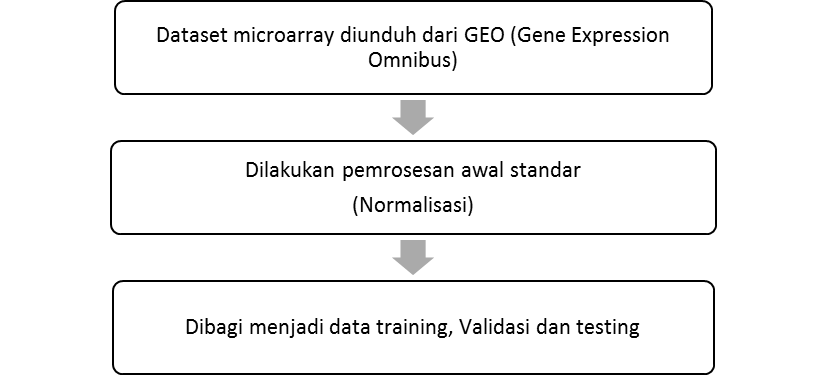
\includegraphics[width=0.9\textwidth]
		{pics/bagian1.png}
	\caption{Proses Pengumpulan data dan Pengolahan Awal}
	\label{fig:pengolahan_awal}
\end{figure}

\subsection{Implementasi dengan R-Bioconductor}
Implementasi preprocessing dengan menggunakan R-Bioconductor

% \lstinputlisting[language=R, frame=single, basicstyle=\tiny]{snip/r_preprocessing.r}


%-----------------------------------------------------------------------------%
\section{Data Profil Gen Percobaan Microarray dan Biomarker}
%-----------------------------------------------------------------------------%

Definisi \textit{Biomarker} adalah sesuatu penanda yang bisa digunakan sebagai indikator suatu penyakit dari pasien. [http://www.biomarker.co.uk/whatisabiomarkers.html] Sebagai contoh, untuk mendiagnosa kanker paru-paru, hanya dibutuhkan 26 ekspresi gen saja. Gen yang paling informatif ini disebut dengan Biomarker (Bing, 2006). Pada profil gen GSE10072 yang merupakan kanker paru-paru, menurut  \citep{belinsky2004gene} ada 26 gen yang paling berpengaruh dari 22.283 gen yang diteliti secara bersamaan, seperti ditunjukkan pada \pic~\ref{fig:biomarker} yang merupakan contoh dari \textit{biomarker} kanker paru-paru.

\begin{figure}
	\centering
	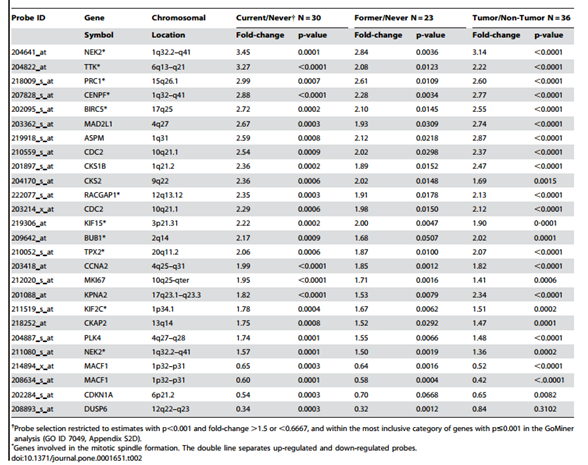
\includegraphics[width=1\textwidth]
		{pics/biomarker.png}
	\caption{Contoh 26 Gen Biomarker Kanker Paru-paru GSE10072}
	\label{fig:biomarker}
\end{figure}


%-----------------------------------------------------------------------------%
\section{Perancangan Metodologi Penelitian}
%-----------------------------------------------------------------------------%

%-----------------------------------------------------------------------------%
\subsection{Tahapan Unsupervised}
%-----------------------------------------------------------------------------%
Tahap \textit{unsupervised} adalah tahapan dimana model DBN ditraining secara \textit{unsupervised} dengan data training pada tiap-tiap layernya secara \textit{greedy}, artinya, proses pelatihan dilakukan secara berjenjang mulai dari layer visibel dengan hidden layer 0 dan kemudian layer ini bobotnya dibuat tetap dan digunakan sebagai input pada leyer berikutnya. Tiap layernya dihitung cost untuk kemudian diminimisasi errornya. Konsep ini disebut \textit{greedy layer-wise training} yaitu setiap layer di traning secara independen dan satu-satu mulai dari layer input yang merupakan data ekspresi gen yang sudah disesuaikan dan dinormalisasi sampai layer output. Seperti pada \pic~\ref{fig:greedy1}

\begin{figure}
	\centering
	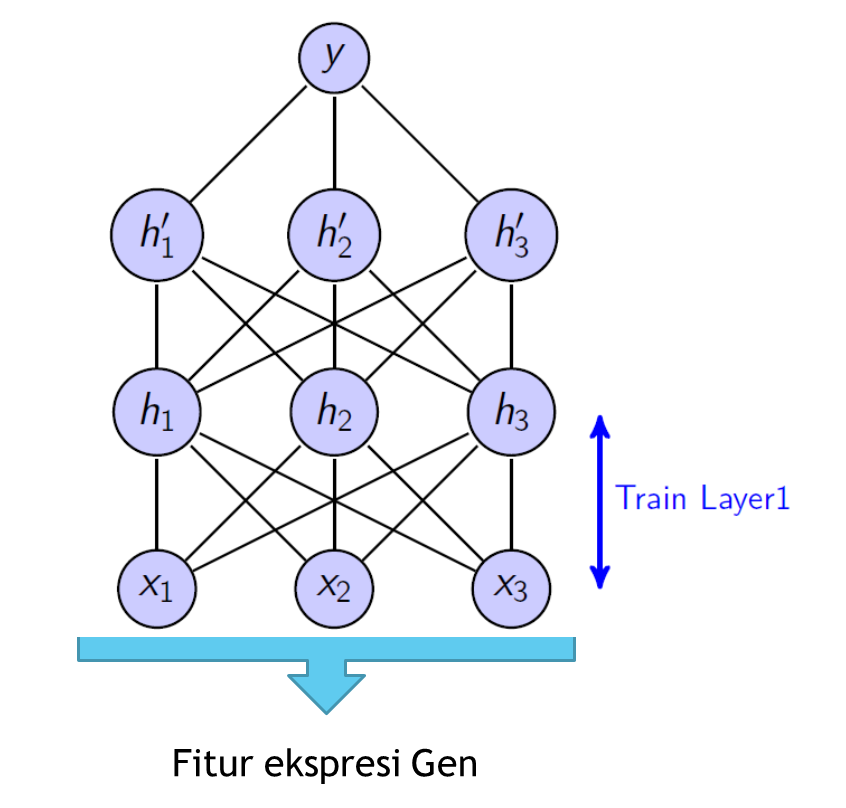
\includegraphics[width=0.5\textwidth]
		{pics/greedy1.png}
	\caption{Greedy layer-wise training pada layer visible dan hidden pertama}
	\label{fig:greedy1}
\end{figure}

Setelah layer pertama selesai di training, layer pertama dibuat \textit{fixed} dan dipakai sebagai inputan visible dari layer selanjutnya. Demikian selanjutnya sampai layer terakhir yaitu layer output. Seperti pada \pic~\ref{fig:greedy2}

\begin{figure}
	\centering
	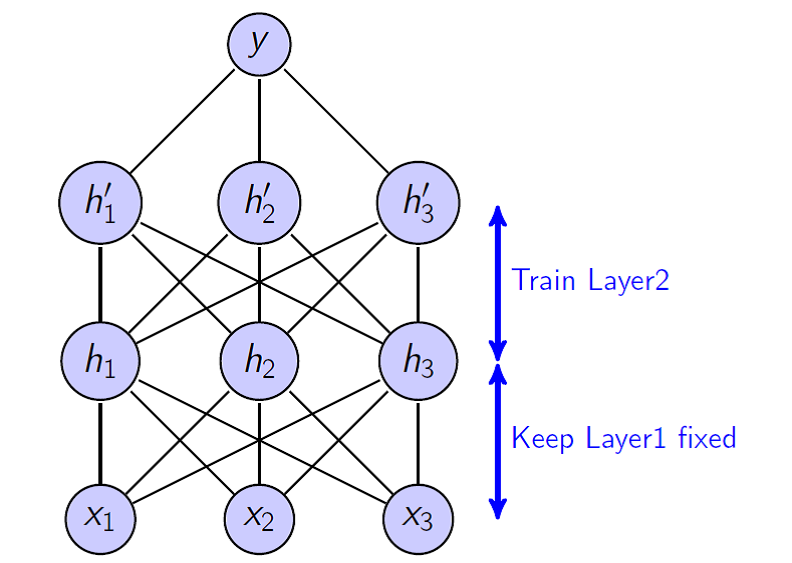
\includegraphics[width=0.5\textwidth]
		{pics/greedy2.png}
	\caption{Greedy layer-wise training pada selanjutnya, yaitu dengan membuat layer sebelumnya Fixed}
	\label{fig:greedy2}
\end{figure}

Pada tahapan training secara unsupervised ini dihitung cost function antara error konstruksi dibandingkan dengan error rekonstruksinya. Dalam RBM yaitu error konstruksi atau disebut error fase positif dibandingkan dengan error rekonstruksi atau error fase negatif.\\
log-likelihood $\mathcal{L}(\theta, \mathcal{D})$ dan fungsi loss-nya sebagai NLL $\ell (\theta, \mathcal{D})$ sebagai berikut:

\begin{equation}
\begin{aligned}
\mathcal{L}(\theta, \mathcal{D}) &= \frac{1}{N} \sum_{x^{(i)} \in
\mathcal{D}} \log\ p(x^{(i)}) \\
\ell (\theta, \mathcal{D}) &= - \mathcal{L} (\theta, \mathcal{D})
\end{aligned}
\end{equation}


Menggunakan stochastic gradient $-\frac{\partial  \log p(x^{(i)})}{\partial
\theta}$, dimana $\theta$ adalah parameter dari modelnya.\\
Loss function merupakan negative log-likelihood dari log-likelihood model. Data dari gradien NLL kemudian memiliki bentuk yaitu:
\begin{equation}
- \frac{\partial  \log p(x)}{\partial \theta}
 = \frac{\partial \mathcal{F}(x)}{\partial \theta} -
       \sum_{\tilde{x}} p(\tilde{x}) \
           \frac{\partial \mathcal{F}(\tilde{x})}{\partial \theta}.
\end{equation}


%-----------------------------------------------------------------------------%
\subsection{Tahapan Supervised}
%-----------------------------------------------------------------------------%
Pada saat \textit{training}  secara \textit{unsupervised} dilakukan, diukur \textit{cost} yang menunjukkan perbedaan antara konstruksi dan rekonstruksi pada tiap layernyanya. Akan tetapi, hal ini hanya untuk mengetahui \textit{cost} tiap-tiap layer RBM-nya, bukan seberapa baik model dalam melakukan klasifikasi. Oleh karena itu diperlukan satu layer output yang yang berupa \textit{logistic regression} untuk mengetahui seberapa baik model dalam membedakan kelas kanker dan bukan kanker.

\subsubsection{Implementasi Logistic Regression pada Layer Output}

Logistic regression adalah klasifier linear yang memiliki matriks bobot $W$ dan vektor bias $b$. Klasifikasi merupakan proyeksi titik data pada sebuah himpunan \textit{hyperplane} yang jaraknya digunakan sebagai penentu probabilitas keanggotaan kelasnya. Secara matematis bisa dituliskan sebagai:
\begin{equation}
\begin{aligned}
  P(Y=i|x, W,b) &= softmax_i(W x + b) \\
                &= \frac {e^{W_i x + b_i}} {\sum_j e^{W_j x + b_j}}
\end{aligned}
\end{equation}

Output dari model akan memprediskikan dengan menghitung \textit{argmax} dari vektor dimana elemen ke $i$ adalah $P(Y=i|x)$.
\begin{equation}
  y_{pred} = argmax_i  P(Y=i|x,W,b)
\end{equation}

Implementasinya menggunakan optimisasi stochastic gradient descent. Untuk implementasi lengkapnya ada di lampiran.

%-----------------------------------------------------------------------------%
\subsection{Tahapan Tuning Parameter}
%-----------------------------------------------------------------------------%
Parameter yang akan dilakukan \textit{tuning} disini adalah: jumlah hidden units, jumlah banyaknya layer hidden dan banyaknya epoch. Tuning parameter dilakukan agar bisa didapatkan hasil yang optimum dari percobaan yang dilakukan. Tahap ini adalah tahap yang paling krusial untuk mendapatkan hasil yang diinginkan. Dikarenakan uniknya data microarray, maka  dilakukan \textit{trial and error} dari parameter-parameternya.\\
Proses tuning parameter ini memerlukan waktu yang lama karena setiap percobaan memiliki parameter yang diubah-ubah untuk menyesuaikan hasil yang diinginkan. Dikarenakan sifat dari microarray yang berbeda dengan citra yang sudah banyak dilakukan oleh peneliti, tuning parameter untuk data \textit{microarray} pada arsitektur deep learning jarang dilakukan oleh peneliti, sehingga proses tuning dilakukan setiap selesai dilakukan percobaan yang memerlukan waktu antara 2 hari sampai 5 hari, tergantung dari epoch dan jumlah layer dan hidden unitnya.\\
Proses training pada arsitektur \textit{deep learning} juga memerlukan kekuatan komputasi komputer yang kuat dan memory yang relatif lebih besar untuk mendapatkan model yang optimal. 



%-----------------------------------------------------------------------------%
\section{Melakukan Testing Arsitektur DBN}
%-----------------------------------------------------------------------------%
Hasil dari unsupervised learning yang dilakukan oleh DBN, akan diuji dahulu dengan dengan data testing, apakah error rekonstruksinya lebih baik. Setelah dilakukan perankingan \textit{biomarker}, diperlukan pengujian apakah apakah seleksi fitur tersebut menggambarkan hasil yang diinginkan, dengan membandingkan biomarker yang dihasilkan dengan literature. 



%-----------------------------------------------------------------------------%
\section{Evaluasi Hasil Perangkingan Dengan Klasifikasi Secara Supervised Menggunakan MLP}
%-----------------------------------------------------------------------------%

Proses evaluasi dilakukan dua kali, pertama, saat menggunakan data asli dan tidak dilakukan seleksi fitur, yang kedua setelah dilakukan seleksi fitur. Hal ini dilakukan untuk mengetahui apakah seleksi fitur tersebut bisa memperbaiki hasil klasifikasi secara signifikan dibandingkan tanpa dilakukan seleksi fitur. \\
Evaluasi hasil hasil perankingan secara \textit{supervised} diperlukan untuk mengetahui apakah hasil perankingan tersebut memperbaiki hasil klasifikasi pasien kanker dan sehat hanya dengan menggunakan gen-gen yang dipilih berdasarkan ranking yang didapatkan.


%-----------------------------------------------------------------------------%
\section{Perbandingan Hasil Perangkingan Dengan Literatur}
%-----------------------------------------------------------------------------%
\begin{figure}
	\centering
	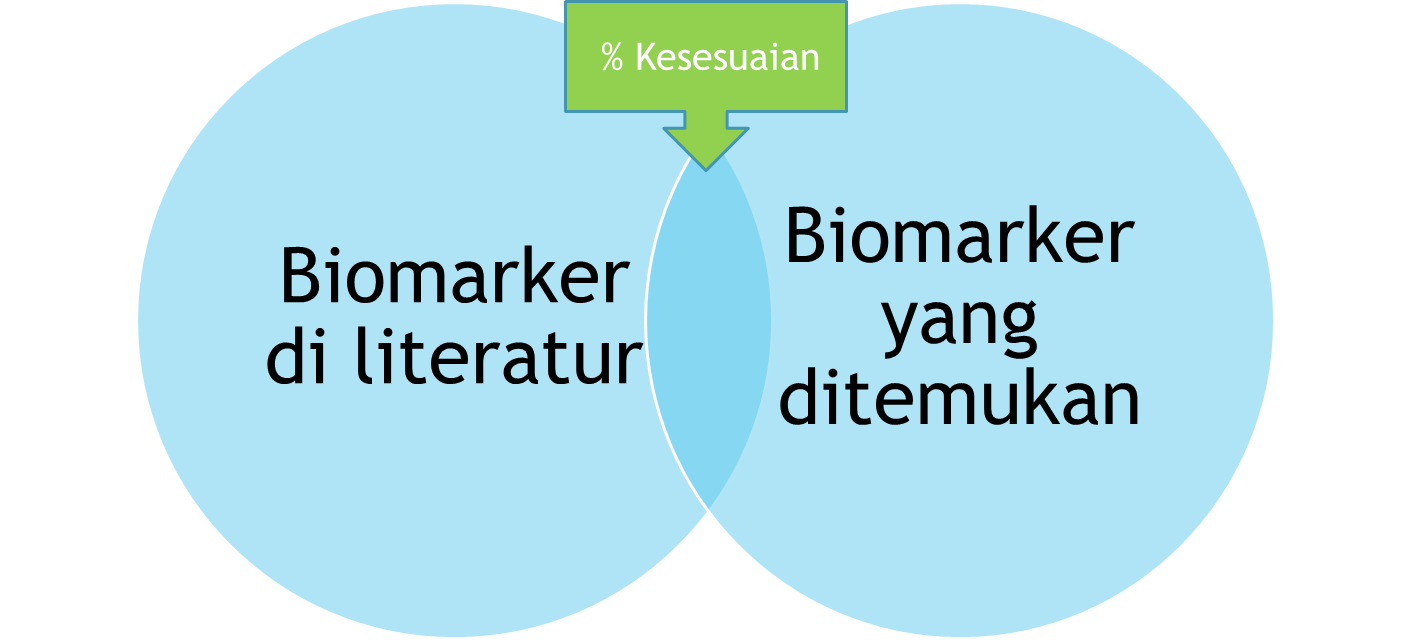
\includegraphics[width=0.9\textwidth]
		{pics/biomarker1.png}
	\caption{Persen Kesesuaian Antara Biomarker yang Ditemukan dibandingkan dengan Biomarker di Literatur}
	\label{fig:biomarker1}
\end{figure}

Hasil perankingan pada percobaan tersebut selanjutnya diteliti apakah gen hasil perankingan tersebut adalah gen yang memiliki signifikansi terhadap penyakit yang diinginkan. Dalam kasus ini yaitu penyakit kanker paru-paru. Berikut adalah contoh 26 gen biomarker pada percobaan GSE10072 yang disitasi dari paper. 

%-----------------------------------------------------------------------------%
\section{Modul-modul Pendukung}
%-----------------------------------------------------------------------------%
\subsection{Kelas Ekstraktor}
Untuk melakukan pengolahan pengolahan awal, didevelop sebuat kelas yang bernama kelas Ekstraktor. Kelas ini berfungsi untuk mengekstrak file csv dari data gen, menjadi file yang memiliki struktur data yang sesuai dengan library dbn.py di python. Hal ini dilakukan agar datanya memiliki struktur yang sesuai dengan dbn yaitu dilakukan normalisasi data profil gen yang berbentuk ekspresi gen menjadi rentang antara 0 sampai 1.

\begin{figure}
	\centering
	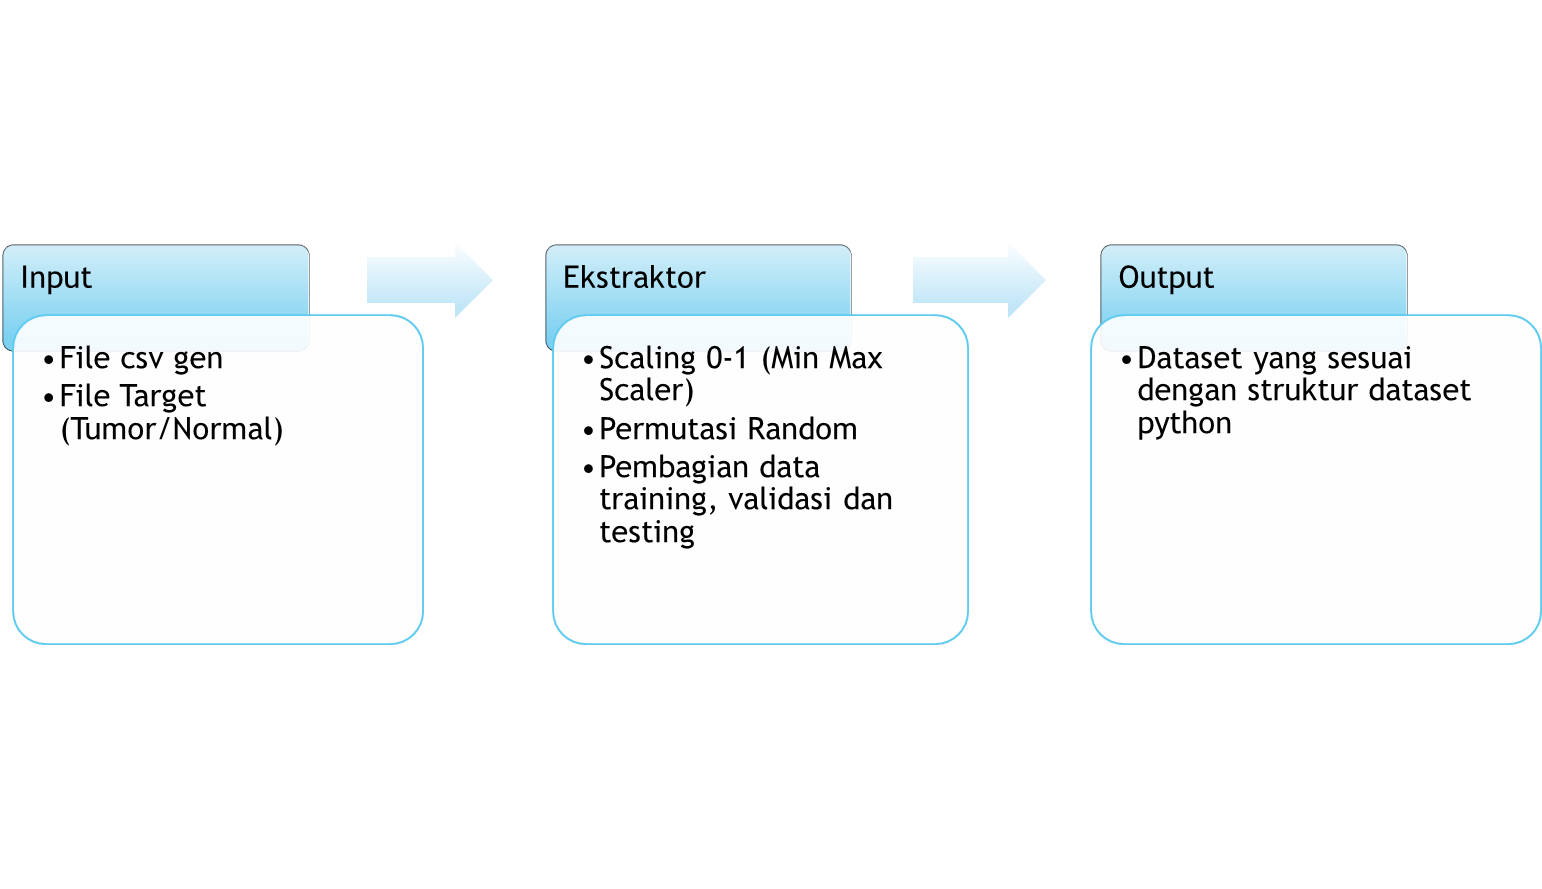
\includegraphics[width=0.9\textwidth]
		{pics/ekstraktor.png}
	\caption{Kelas Ekstraktor, Untuk melakukan Ekstraksi data Gen}
	\label{fig:preproses}
\end{figure}

\subsection{Implementasi Kelas Ekstraktor di Python}
Listing 4.1: Ekstraksi dataset untuk disesuaikan dengan struktur data modul dbn.py
\lstinputlisting[language=python, frame=single, basicstyle=\tiny]{snip/ekstrak_csv.py}

Kelas ekstraktor ini melakukan adaptasi data yang tadinya memiliki struktur yang tidak kompatibel dengan library Theano yang di python, menjadi kompatibel dan memiliki struktur data yang disesuaikan. Kemudian, dilakukan juga permutasi random agar datanya memiliki sebaran yang normal untuk kemudian dilakukan pembagian data yang terdiri dari sekian persen data training, validasi dan testing.

\subsection{Kelas Generator}
Kelas Generator ini adalah modul yang dibuat agar bisa secara otomatis memilih gen-gen yang dianggap penting pada sebuah array yang berisi index dari gen yang ada pada dataset.
\begin{figure}
	\centering
	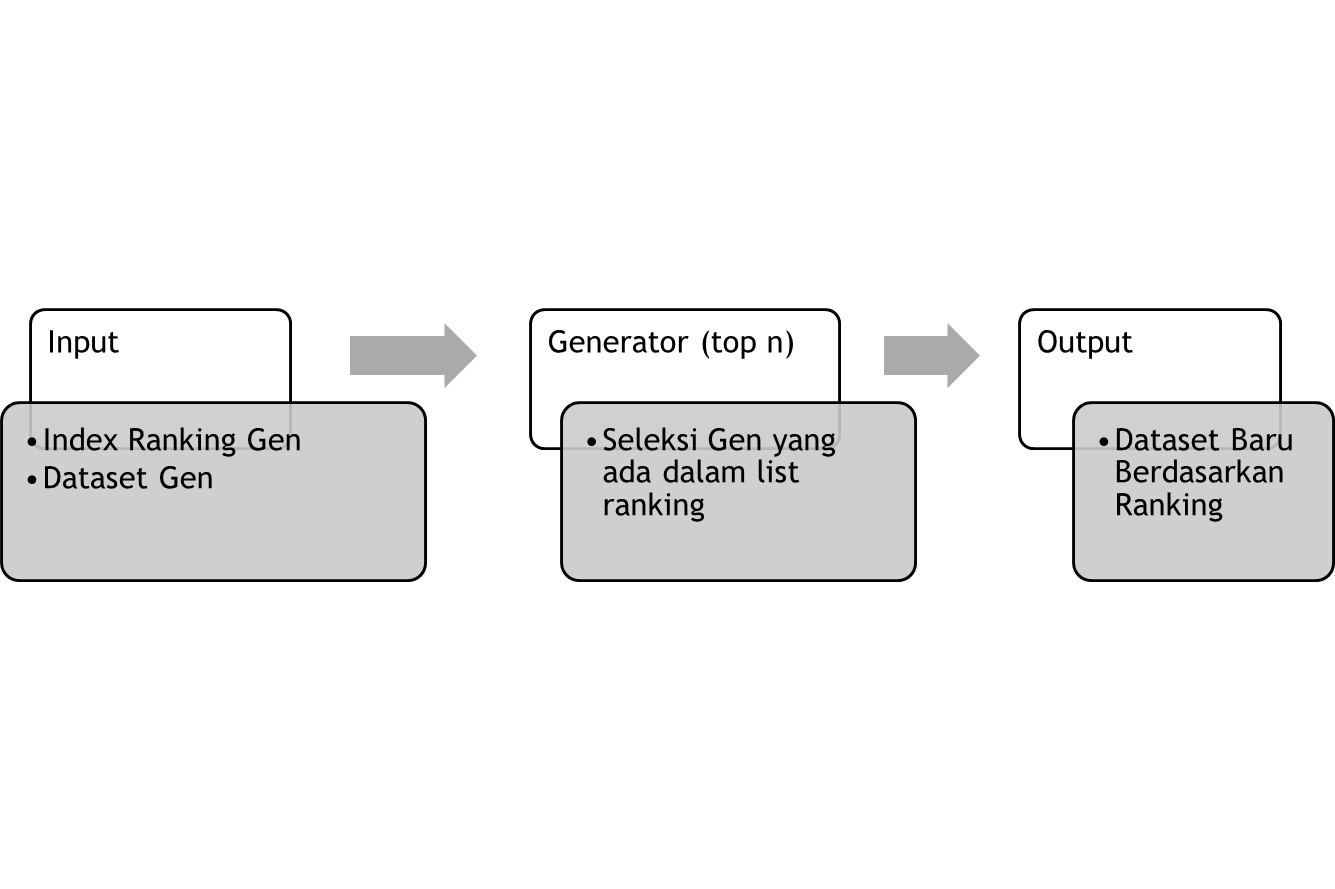
\includegraphics[width=0.8\textwidth]
		{pics/generator.png}
	\caption{Diagram Kelas Generator yang digunakan untuk menggenerasi data gen berdasarkan rankingnya}
	\label{fig:generator}
\end{figure}


\subsection{Hasil Evaluasi Dengan Multi Layer Perceptron}

\begin{figure}
	\centering
	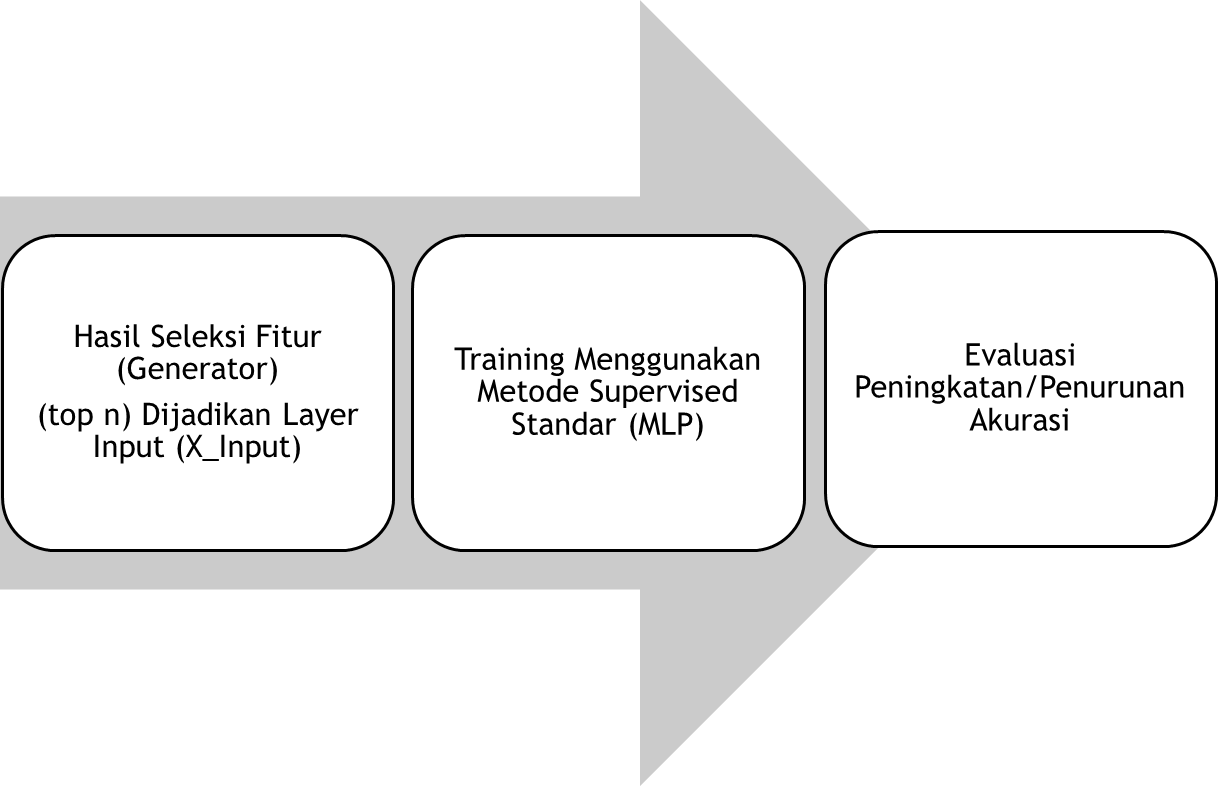
\includegraphics[width=0.7\textwidth]
		{pics/generator2.png}
	\caption{Diagram Proses Menggenerasi Data Untuk Dijadikan Dataset Training}
	\label{fig:generator2}
\end{figure}







%-----------------------------------------------------------------------------%
\chapter{\babEmpat}
%-----------------------------------------------------------------------------%

Pada bab 4 ini akan dibahas tentang hasil penelitian dari metodologi yang ada pada bab tiga, dan masalah-masalah yang dihadapi pada saat implementasinya dan pembahasannya.


%-----------------------------------------------------------------------------%
\section{Overview Metodologi}
%-----------------------------------------------------------------------------%
Model yang dihasilkan dari \textit{unsupervised learning} yang dilakukan oleh DBN menggunakan data training, harus diuji dahulu dengan dengan data validasi dan data testing, yaitu dengan cara memberikan satu layer output menggunakan \textit{logistic regression} hal ini untuk mengetahui apakah klasifikasinya lebih baik atau sebaliknya. Hasil ini berpengaruh pada proses tuning parameter (jumlah layer dan jumlah hidden unitnya) untuk didapatkan \textit{cost} yang paling optimal pada saat pre-training. Setelah dilakukan perankingan secara multi-step dari hasil percobaan yang terbaik, diperlukan pengujian apakah apakah seleksi fitur tersebut mendapatkan hasil klasifikasi yang lebih baik dengan menggunakan fitur yang telah diseleksi saja. Dengan cara membandingkan \textit{biomarker} yang ditemukan oleh algoritma multi-step rangking dibandingkan dengan algoritma yang ada di literatur yaitu metode \textit{bonferroni} untuk melakukan test statistik pada data gen tersebut \citep{hochberg1988sharper}. 


%-----------------------------------------------------------------------------%
\section{Hasil Percobaan DBN Dengan Setting Hyperparameter yang Berbeda}
%-----------------------------------------------------------------------------%
Untuk mendapatkan hasil yang optimal dibutuhkan banyak percobaan dan setting parameter yang berbeda-beda, mulai dari jumlah layer, jumlah hidden unit tiap layernya, learning rate dan ukuran batch-nya. Oleh karena itu, dibawah adalah rekapitulasi percobaan dengan hasil terbaik dari sekian percobaan, dipilih lima percobaan yang paling baik hasilnya untuk kemudian dianalisa lebih jauh. Percobaan dibawah memiliki setting parameter seperti pada daftar berikut:


% Please add the following required packages to your document preamble:
% \usepackage{booktabs}
\begin{table}
\centering
\caption{Setting Parameter Awal}
\label{tab:var}
\begin{tabular}{@{}lll@{}}
\toprule
No. & Item          & Keterangan                                                                                                                                                \\ \midrule
1   & Dataset       & \begin{tabular}[c]{@{}l@{}}Gene expression signature of cigarette smoking \\ and its role in lung adenocarcinoma development \\ and survival \citep{landi2008gene} \end{tabular} \\
2   & Total Data    & 107 Pasien                                                                                                                                                \\
3   & Kanker        & 58 Pasien                                                                                                                                                 \\
4   & Normal        & 49 Pasien                                                                                                                                                 \\
5   & Training      & 69 Pasien                                                                                                                                                 \\
6   & Validasi      & 15 Pasien                                                                                                                                                 \\
7   & Testing       & 23 Pasien                                                                                                                                                 \\
8   & Epoch         & 1000 dan 2000                                                                                                                                             \\
9   & Learning Rate & 0.01                                                                                                                                                      \\
10  & Fitur Gen     & 22.283 Gen                                                                                                                                                \\ \bottomrule
\end{tabular}
\end{table}
Setelah dilakukan eksperimen secara \textit{unsupervised} diperoleh \textit{cost} terbaik pada Percobaan dan hasilnya ada di tabel \ref{tab:dbn} :


\begin{table}
\centering
\caption{Eksperimen DBN Unsupervised}
\label{tab:dbn}
\tabcolsep=0.11cm
\begin{tabular}{@{}llllllll@{}}
\toprule
\multicolumn{1}{c}{Eks} & \multicolumn{1}{c}{Hidden} & \multicolumn{1}{c}{Epoch} & \multicolumn{1}{c}{Cost Lyr 0} & \multicolumn{1}{c}{Cost Lyr 1} & Cost Lyr 2 & Cost Lyr 3 & Waktu (Jam) \\ \midrule
1 & \begin{tabular}[c]{@{}l@{}}{[}10000, 5000,\\  1000, 500{]}\end{tabular} & 1000 & -12888.2 & -1.37401 & -3499.73 & -0.351105 & 65 \\
 &  & 2000 & -12888.2 & -0.828167 & -3484.73 & -0.150991 & 132 \\
2 & \begin{tabular}[c]{@{}l@{}}{[}7000, 10000, \\ 5000, 1000{]}\end{tabular} & 1000 & -12886.8 & -1.36201 & -6866.37 & -0.163702 & 63 \\
 &  & 2000 & -12886.7 & -1.57877 & -6873.31 & -0.0729352 & 138 \\
3 & \begin{tabular}[c]{@{}l@{}}{[}3000, 2000, \\ 1000, 100{]}\end{tabular} & 1000 & -12897.8 & -0.862442 & -1410.18 & -3.244 & 58 \\
 &  & 2000 & -12897.0 & -0.849616 & -1397.09 & -3.14657 & 123 \\
4 & \begin{tabular}[c]{@{}l@{}}{[}15000, 8000, \\ 2000{]}\end{tabular} & 1000 & -12934.5 & -32.4227 & -2756.41 & (null) & 68 \\
5 & \begin{tabular}[c]{@{}l@{}}{[}25000, 17000, \\ 7000{]}\end{tabular} & 1000 & -12888.1 & -12.1715 & -5446.34 & (null) & 72 \\ \bottomrule
\end{tabular}
\end{table}



Tabel diatas menunjukkan bahwa dengan epoch 1000 dan 2000 costnya tidak menunjukkan perbaikan secara signifikan. Bahkan untuk beberapa kasus, hasilnya lebih buruk. Dibawah adalah plot cost untuk percobaan yang dilakukan secara \textit{greedy layer wise}, dari plot tersebut dapat dilihat bahwa cost pada epoch 700-an sudah tidak lagi membaik secara signifikan. Hal ini bisa dikarenakan oleh terbatasnya data training yang dipakai yaitu hanya 69 pasien dikarenakan oleh terbatasnya data yang didapatkan karena mahalnya percobaan microarray itu sendiri.

\subsection{Plot Cost Percobaan 1 (Hidden = [10k, 5k, 1k, 500])}

\begin{figure}
	\centering
	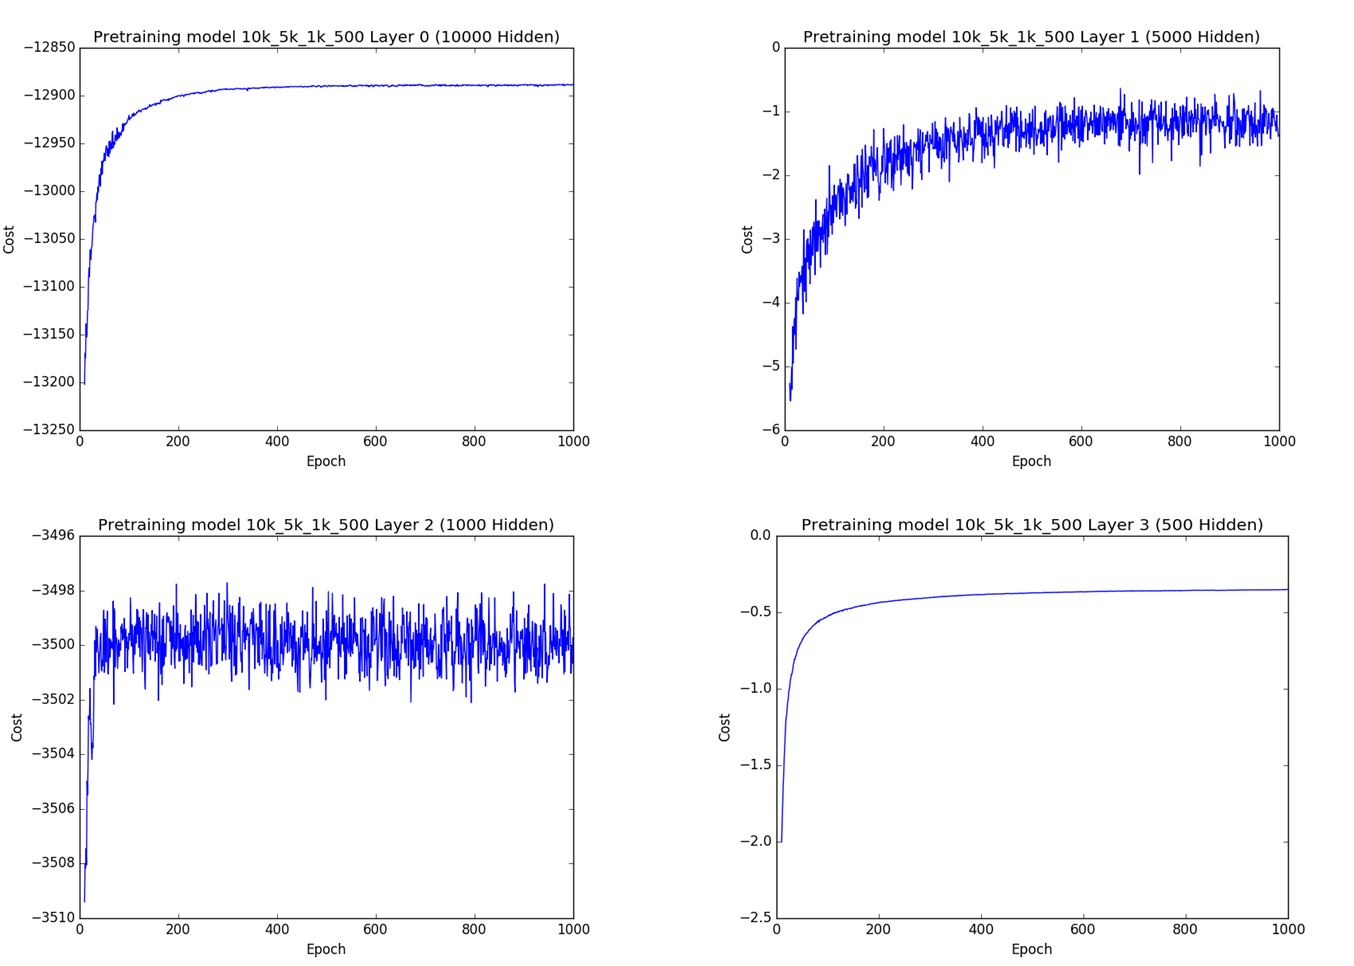
\includegraphics[width=0.9\textwidth]
		{pics/percobaan_1.png}
	\caption{Perbandingan Cost Pada Percobaan 1 Sampai 1000 Epoch Pada Tiap Layernya}
	\label{fig:percobaan1}
\end{figure}

Pada \pic~\ref{fig:percobaan1} merupakan perbandingan cost dari layer 0 sampai 3 (4 layer) dengan konfigurasi hidden [10000, 5000,1000,500] disitu bisa dilihat bahwa setelah epoch 500 tidak terjadi perbaikan cost yang signifikan. Juga cost pada layer 2 dan 3 memiliki ritme yang tidak stabil.

\subsection{Plot Cost Percobaan 2 (Hidden = [7k, 10k, 5k, 1k])}
\begin{figure}
	\centering
	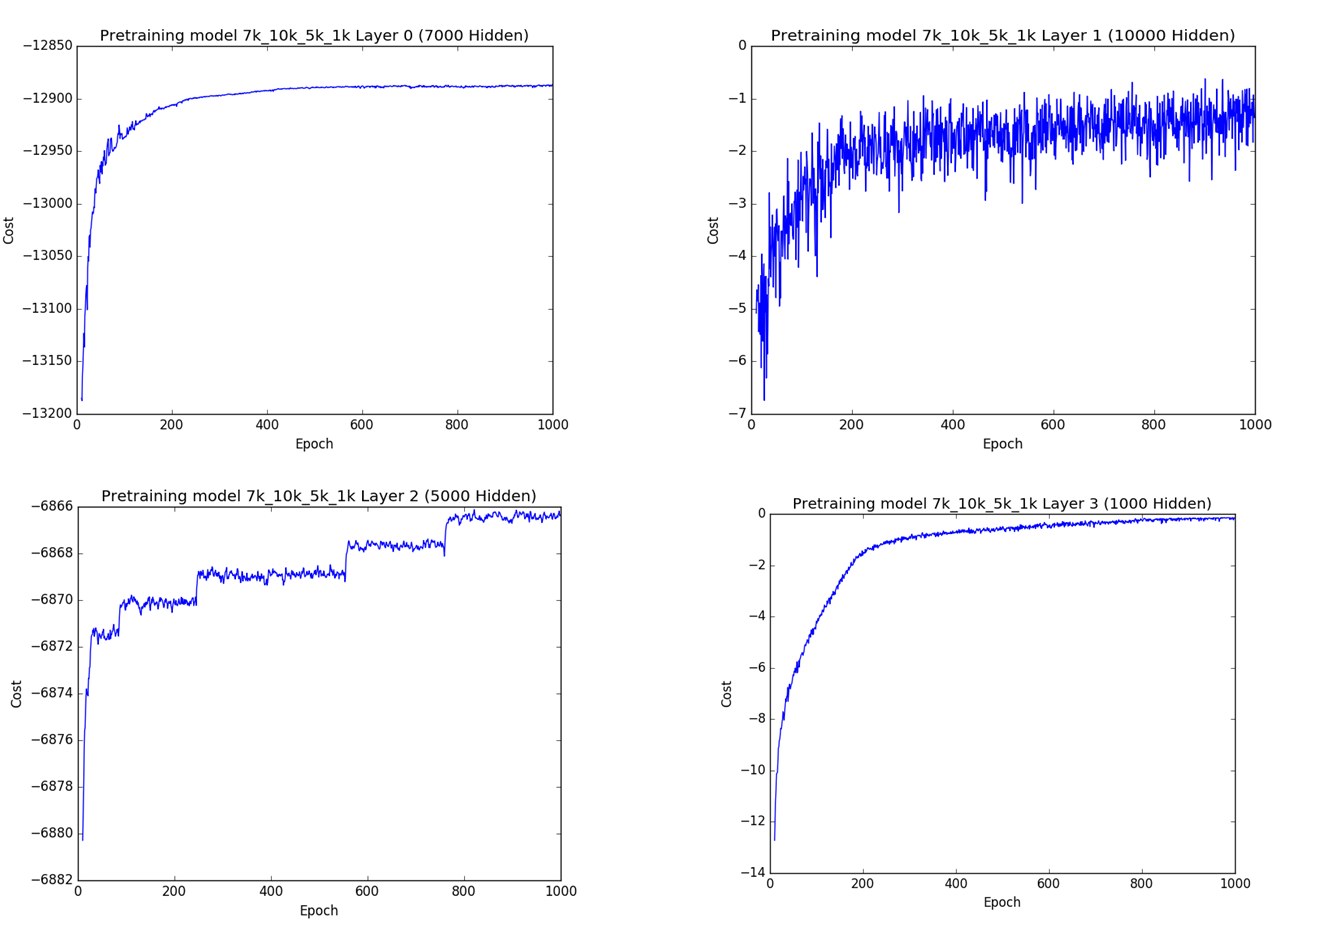
\includegraphics[width=0.9\textwidth]
		{pics/percobaan_2.png}
	\caption{Perbandingan Cost Pada Percobaan 2 Sampai 1000 Epoch Pada Tiap Layernya}
	\label{fig:percobaan2}
\end{figure}

Pada \pic~\ref{fig:percobaan2} merupakan perbandingan cost dari layer 0 sampai 3 (4 layer) disitu bisa dilihat bahwa setelah epoch 500 tidak terjadi perbaikan cost yang signifikan. Juga cost pada layer 2 dan 3 memiliki ritme yang juga tidak stabil.

\subsection{Plot Cost Percobaan 3 (Hidden = [3k, 2k, 1k, 100])}
\begin{figure}
	\centering
	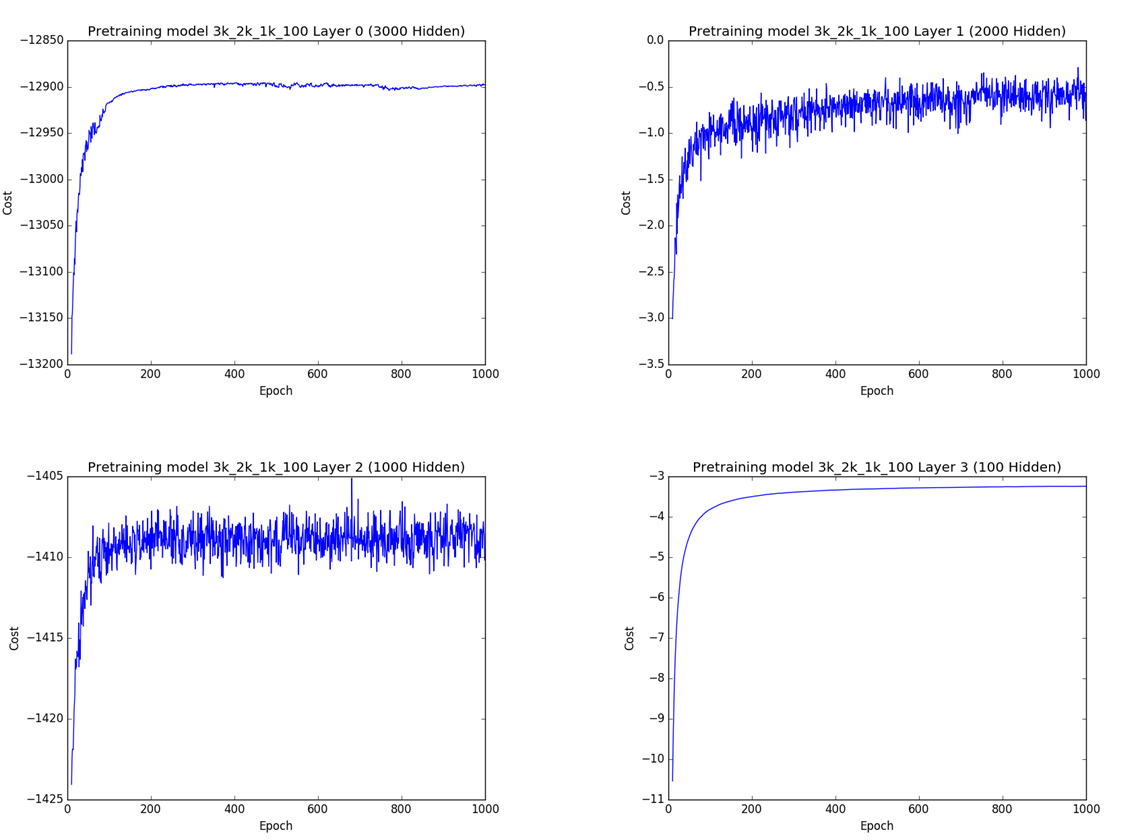
\includegraphics[width=0.9\textwidth]
		{pics/percobaan_3.png}
	\caption{Perbandingan Cost Pada Percobaan 3 Sampai 1000 Epoch Pada Tiap Layernya}
	\label{fig:percobaan3}
\end{figure}
Pada \pic~\ref{fig:percobaan3} merupakan perbandingan cost dari layer 0 sampai 3 (4 layer) disitu bisa dilihat bahwa setelah epoch 700-an tidak terjadi perbaikan cost yang signifikan. Juga \textit{cost} pada layer 2 dan 3 memiliki ritme yang tidak stabil.

Berarti dari ketiga percobaan tersebut, secara garis besar, epoch lebih dari 700-an tidak mempengaruhi perbaikan error rekonstruksinya. Hal ini bisa disebabkan karena kurangnya data training.


%-----------------------------------------------------------------------------%
\section{Hasil Penerapan Multi Step Ranking Bobot}
%-----------------------------------------------------------------------------%

Percobaan training DBN secara \textit{unsupervised} yang dilakukan dengan setting pada tabel \ref{tab:dbn} diatas dipilih tiga percobaan terbaik untuk dilakukan algoritma multi-step ranking.

\subsection{Diagram Venn Perpotongan Percobaan 1, 2 dan 3}

Pada saat dilakukan multi-step ranking pada percobaan 1, 2 dan 3. Dibuat perankingan top 250 gen yang paling berpengaruh terhadap model-nya masing-masing. Kemudian, dibuat sebuah diagram untuk mendapatkan perpotongan 250 gen tersebut pada tiap-tiap percobaan. Hal ini digunakan untuk mengetahui gen-gen mana yang selalu muncul di percobaan 1,2,3 atau muncul di dua percobaan dan hanya muncul di satu percobaan. Maka didapatkan diagram venn seperti pada \pic~\ref{fig:venn1}

\begin{figure}
	\centering
	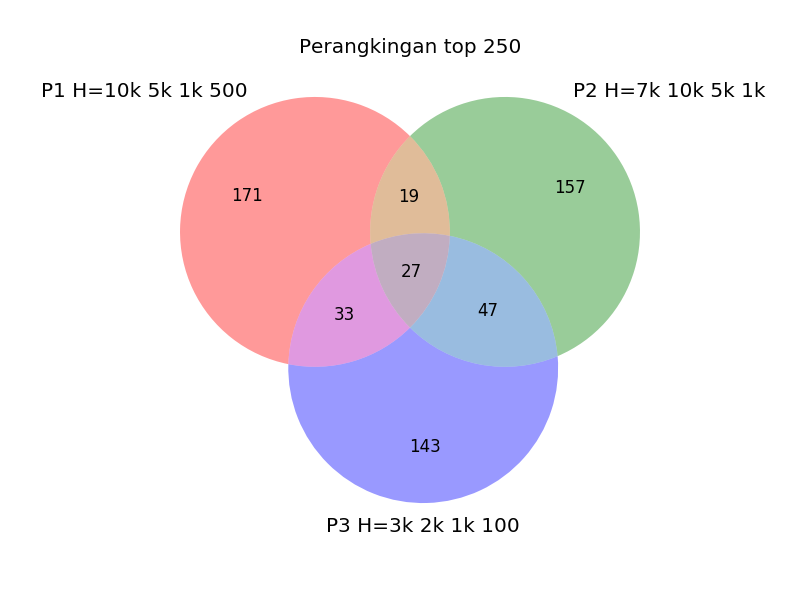
\includegraphics[width=0.9\textwidth]
		{pics/venn1.png}
	\caption{Perbandingan Perankingan Top 250 pada tiga percobaan yang paling baik, ada 27 gen yang selalu muncul pada ketiga percobaan tersebut}
	\label{fig:venn1}
\end{figure}
Pada diagram venn diatas, ditunjukkan bahwa ada 27 gen yang selalu muncul pada percobaan 1, 2, 3. Hal ini menunjukkan bahwa gen tersebut adalah gen yang diindikasikan lebih informatif dibandingkan dengan gen yang lainnya. Ke 27 gen tersebut ada pada tabel \ref{tab:indexgen} penemuan 27 gen yang selalu muncul pada tiga percobaan terbaik tersebut bisa diindikasikan sebagai \textit{biomarker}. Yaitu gen yang bisa mencirikan seseorang terkena kanker paru-paru atau tidak.\\


% Please add the following required packages to your document preamble:
% \usepackage{booktabs}
\begin{table}
\centering
\caption{Index dan Kode Gen yang Diindikasikan sebagai \textit{Biomarker}}
\label{tab:indexgen}
\begin{tabular}{@{}ll@{}}
\toprule
Index & Kode Gen      \\ \midrule
7303  & 207783\_x\_at \\
1418  & 201891\_s\_at \\
9666  & 210183\_x\_at \\
15890 & 216520\_s\_at \\
24    & 200004\_at    \\
21919 & 38691\_s\_at  \\
11298 & 211911\_x\_at \\
13741 & 214363\_s\_at \\
46    & 200026\_at    \\
307   & 200780\_x\_at \\
12727 & 213347\_x\_at \\
13246 & 213867\_x\_at \\
4418  & 204892\_x\_at \\
6084  & 206559\_x\_at \\
13765 & 214387\_x\_at \\
328   & 200801\_x\_at \\
201   & 200674\_s\_at \\
21860 & 37004\_at     \\
101   & 200081\_s\_at \\
232   & 200705\_s\_at \\
11370 & 211984\_at    \\
879   & 201352\_at    \\
11120 & 211720\_x\_at \\
20968 & 221607\_x\_at \\
115   & 200095\_x\_at \\
1019  & 201492\_s\_at \\
511   & 200984\_s\_at \\ \bottomrule
\end{tabular}
\end{table}

Ke-27 gen pada tabel tersebut merupakan gen yang diindikasikan memiliki pengaruh yang signifikan pada percobaan. Akan tetapi hal ini perlu dilakukan konfirmasi lebih lanjut untuk memastikan bahwa gen tersebut memang berpengaruh secara signifikan terhadap penyakit kanker paru-paru. Ada dua tahapan konfirmasi yang pertama tahap konfirmasi dengan memastikan bahwa hasil klasifikasi dengan hanya menggunakan top 250 gen tersebut bisa mengklasifikasikan pasien sehat dan pasien kanker. Tahap yang kedua adalah dengan cara konfirmasi melalui literatur tentang biomarker kanker paru-paru yang sudah ditemukan pada penelitian sebelumnya.

%-----------------------------------------------------------------------------%
\section{Bagian Supervised Learning Dengan Multi Layers Perceptron (MLP)}
%-----------------------------------------------------------------------------%

Pada saat dilakukan klasifikasi pasien kanker dan normal tanpa dilakukan seleksi fitur, dikarenakan banyaknya fitur gen yang merupakan noise, maka perbandingan fitur gen dan pasien menjadi sangat lebar, oleh karena itu sangat rentan dengan masalah yang sering timbul dari teknik pembelajaran mesin yaitu \textit{overfitting}. Oleh karena itu, salah satu cara untuk menghindari overfitting adalah dengan metode seleksi fitur. \\
Setelah dilakukan perbandingan gen biomarker yang ditemukan pada proses perankingan diatas, top 250 gen tersebut dibuat menjadi data input untuk kasus klasifikasi. Untuk di evaluasi apakah hasil klasifikasinya lebih baik dibandingkan dengan tanpa seleksi fitur.\\
Tabel \ref{tab:tabel4.2} merupakan perbandingan error antara logistic regression yang ditempatkan pada layer akhir DBN, tanpa dilakukan seleksi fitur. Dibandingkan dengan MLP yang memiliki 1 layer hidden dan 250 hidden unit. Untuk dilakukan training ulang dan dibandingkan dengan hasil yang diperoleh dari logistic regression.

\begin{table}
\centering
\caption{Perbandingan Error Antara Dengan dan Tanpa Seleksi Fitur}
\label{tab:tabel4.2}
\begin{tabular}{@{}lllll@{}}
\toprule
 & \multicolumn{2}{l}{Tanpa Seleksi Fitur(LogReg)} & \multicolumn{2}{l}{Dengan Seleksi Fitur(MLP)} \\ \midrule
Percobaan & Validation Error & Test Error & Validation Error & Test Error \\
1 & 50\% & 66\% & 5.55\% & 0\% \\
2 & 50\% & 30\% & 0\% & 8.33\% \\
3 & 50\% & 30\% & 0\% & 16\% \\ \bottomrule
\end{tabular}
\end{table}

Dari tabel \ref{tab:tabel4.2} dapat disimpulkan bahwa terjadi perbaikan signifikan antara validation dan test error dibandingkan tanpa dilakukan seleksi fitur. Akan tetapi hal ini masih belum menunjukkan apakah seleksi fitur gen tersebut merupakan \textit{biomarker}. Oleh karena itu diperlukan evaluasi lebih lanjut yaitu dengan evaluasi literatur untuk memastikan bahwa gen yang ditemukan memang informatif untuk kasus kanker paru-paru.

%-----------------------------------------------------------------------------%
\section{Hasil Evaluasi Dengan Literatur Pertama Bonferroni Method\citep{hochberg1988sharper}}
%-----------------------------------------------------------------------------%

Metode Bonferroni adalah metode multipel testing di statistik yang paling umum digunakan untuk dataset dari percobaan \textit{microarray}. Metode ini adalah metode yang dipakai oleh \cite{landi2008gene} dalam menganalisa dataset GSE10072 yang merupakan hasil eksperimen kanker paru-paru \citep{landi2008gene} Dengan melakukan test statistik menggunakan metode bonferroni dipilih 250 gen yang paling signifikan dari hasil test statistik tersebut dibandingkan dengan gen yang dipilih dari metode multi-step ranking, didapatkan hasil sebagai berikut.

\begin{figure}
	\centering
	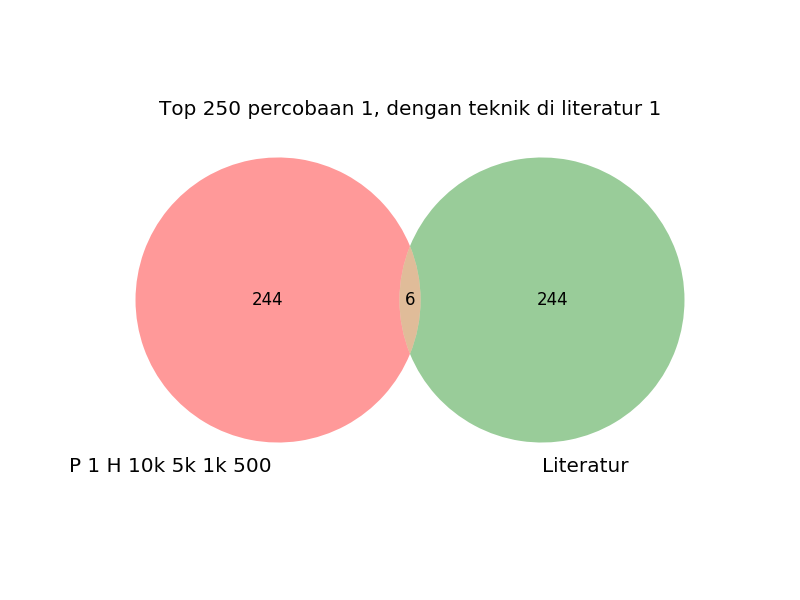
\includegraphics[width=0.9\textwidth]
		{pics/bon1.png}
	\caption{Hasil top 250 Gen dibandingkan dengan Metode bonferroni}
	\label{fig:bon1}
\end{figure}

Pada percobaan 1, dihasilkan perpotongan 6 gen. Walaupun kelihatan kecil tetapi perpotongan 6 gen dari 22 ribu-an gen menjadi sangat signifikan untuk diteliti lebih lanjut gen-gen tersebut sebagai kandidat \textit{Biomarker}

\begin{figure}
	\centering
	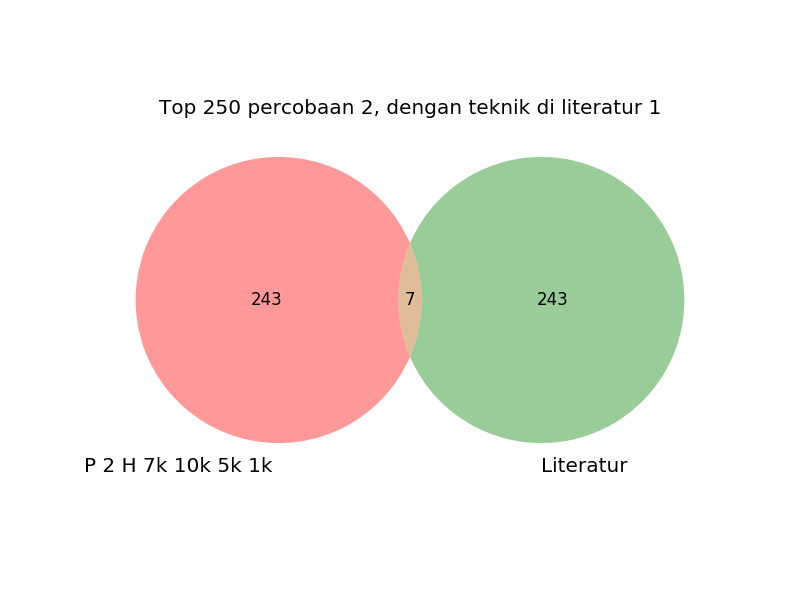
\includegraphics[width=0.9\textwidth]
		{pics/bon2.png}
	\caption{Hasil top 250 Gen dibandingkan dengan Metode bonferroni}
	\label{fig:bon1}
\end{figure}

Percobaan 2 dibandingkan dengan metode bonferroni juga memiliki perpotongan yang tidak besar yaitu 7 gen saja.

\begin{figure}
	\centering
	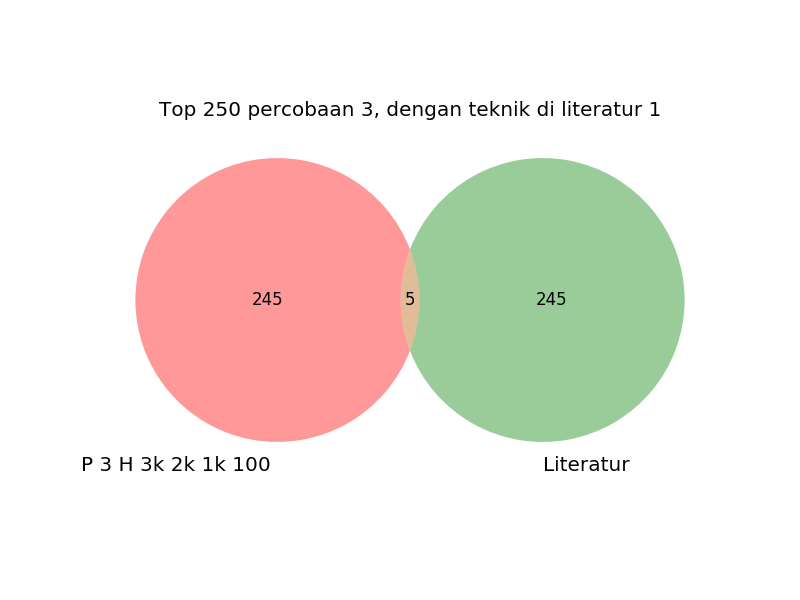
\includegraphics[width=0.9\textwidth]
		{pics/bon3.png}
	\caption{Hasil top 250 Gen dibandingkan dengan Metode bonferroni}
	\label{fig:bon3}
\end{figure}

Percobaan 3 dibandingkan dengan metode bonferroni memiliki perpotongan kesesuaaina 5 gen.



%-----------------------------------------------------------------------------%
\section{Hasil Konfirmasi Dengan Literatur Kedua Harvard Cancer Center (https://ccib.mgh.harvard.edu/xavier)}
%-----------------------------------------------------------------------------%
Sebanyak 27 gen yang ditemukan untuk irisan tiga percobaan terbaik, akan dilakuan review literatur lebih jauh. Menurut situs harvard cancer center, gen-gen tertentu bisa menununjukkan tingkat signifikansi gen tersebut terhadap sebuah penyakit kanker. Gen yang berada pada ranking 1 sampai 27 tersebut memiliki signifikasni yang tinggi terhadap kanker paru-paru dibandingkan dengan gen yang dipilih secara acak.
\begin{figure}
	\centering
	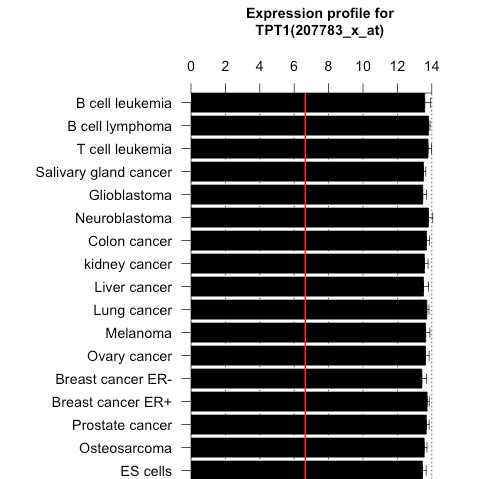
\includegraphics[width=0.9\textwidth]
		{pics/tpt1.png}
	\caption{Profil Ekspresi Gen TPT1 yang merupakan ranking pertama}
	\label{fig:tpt1}
\end{figure}
Dari gambar bisa dilihat bahwa signifikansi gen TPT1 yang merupakan gen dengan ranking pertama memiliki signifikansi terhadap penyakit kanker paru-paru (lung cancer). Sumber profil gen didapat dari https://ccib.mgh.harvard.edu/xavier

\begin{figure}
	\centering
	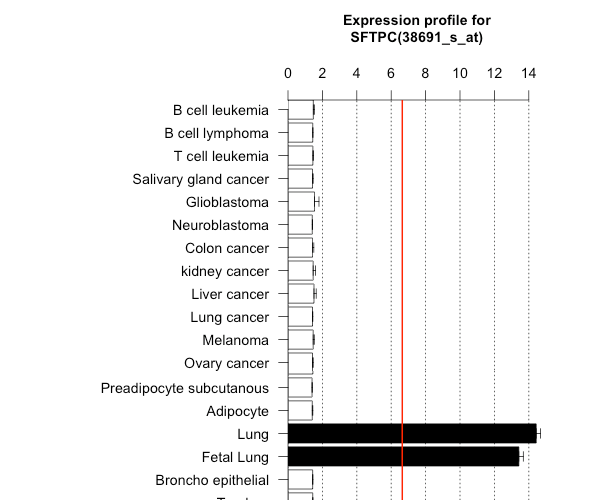
\includegraphics[width=0.9\textwidth]
		{pics/38691_s_at_profil.png}
	\caption{Profil Ekspresi Gen TPT1 yang merupakan ranking pertama}
	\label{fig:SFTPC}
\end{figure}

Pada dua contoh profil yang ditemukan yaitu gen TPT1 dan gen SFTPC bisa disimpulkan bahwa walaupun ekspresi gen tersebut ditemukan pada kanker paru-paru, tetapi tidak unik dan juga ditemukan di kanker-kanker yang lain misalnya leukemia, lymphoma dan sebagainya. Hal ini terjadi karena data yang dipakai adalah data kanker paru-paru saja. Sehingga gen yang sama bisa signifikan pada kanker-kanker lainnya dikarenakan tidak adanya data selain kanker paru-paru untuk dijadikan data trainingnya.
%-----------------------------------------------------------------------------%
\section{Kendala-Kendala yang Dialami Selama Melakukan Percobaan}
%-----------------------------------------------------------------------------%
Pada saat melakukan percobaan dengan menggunakan arsitektur \textit{deep learning} kendala yang paling utama adalah lamanya waktu training dan penggunaan resource memory yang sangat besar. Dengan menggunakan komputer core i5 dengan memory vga 2 GB, dan RAM 4 GB diperlukan waktu rata-rata 3-5 hari. Seperti pada tabel \ref{tab:runtime}. Dikarenakan oleh kendala ini maka untuk melakukan percobaan dengan arsitektur yang lebih besar, misalnya dilakukan penambahan layer (lebih dari 4 layer) dan penambahan hidden unit, menjadi terbatas. Juga masalah pada terbatasnya dataset untuk training yang hanya 107 sampel pasien, hal ini disebabkan oleh mahalnya percobaan \textit{microarray} yang dilakukan sehingga sulit untuk mendapatkan data yang lebih besar lagi.

\begin{table}
\centering
\caption{tabel ukuran model dan waktu running}
\label{tab:runtime}
\begin{tabular}{@{}llll@{}}
\toprule
Percobaan & \begin{tabular}[c]{@{}l@{}}Konfigurasi Hidden\\ (h0, h1, h2, h3)\end{tabular} & Ukuran Model  & \begin{tabular}[c]{@{}l@{}}Running (Jam)\\ (1000e, 2000e)\end{tabular} \\ \midrule
1         & 10000, 5000,1000, 500                                                         & 1 GB          & 65, 132                                                                \\
2         & 7000,10000,5000,1000                                                          & 1 GB          & 63, 138                                                                \\
3         & 3000,2000,1000,100                                                            & 275 MB        & 58, 123                                                                \\
4         & 15000,8000,2000                                                               & Out of Memory & -                                                                      \\
5         & 25000, 17000, 7000                                                            & Out of Memory & -                                                                      \\ \bottomrule
\end{tabular}
\end{table}

Pada tabel diatas, bisa dihilhat bahwa hidden yang melebihi 15000 sudah menghabiskan RAM komputer yang hanya berukuran 4 GB. Oleh karena itu, percobaan yang seharusnya bisa memperdalam layer dan memperbesar hidden unit tidak memungkinkan untuk dilakukan.






%---------------------------------------------------------------
\chapter{\kesimpulan}
%---------------------------------------------------------------
	

%---------------------------------------------------------------
\section{Kesimpulan}
%---------------------------------------------------------------
Penelitian ini menerapkan seleksi fitur perankingan multi-step pada \textit{arsitektur deep believe network (DBN)} untuk mencari \textit{biomarker} pada data microarray penyakit kanker paru-paru. Penerapannya menggunakan library Theano pada bahasa pemrograman Python. Kesimpulan yang dapat diambil dari penelitian ini adalah sebagai berikut:
\begin{enumerate}
\item Metodologi pencarian \textit{biomarker} secara \textit{unsupervised} dengan menggunakan teknik \textit{Deep Believe Network (DBN)} didapatkan model terbaik  dengan konfigurasi hidden unit 4 layer [7000, 10000, 5000, 1000] dengan epoch 1000 dan learning rate 0.01.
\item Algoritma perankingan gen secara multi-step pada jaringan DBN yang merupakan modifikasi dari metode sebelumnya yang hanya bisa dilakukan pada teknik \textit{logistic regression} sekarang bisa dilakukan untuk network DBN yang di training secara \textit{unsupervised} murni.
\item Evaluasi yang dilakukan secara bertahap yaitu mulai dari dibandingkannya metode unsupervised dengan masalah klasifikasi \textit{supervised} dengan MLP menunjukkan peningkatan hasil klasifikasi yang signifikan. Dan \textit{biomarker} yang ditemukan, dibandingkan dengan literatur yaitu metode bonferroni menunjukkan bahwa gen yang ditemukan memiliki signifikansi yang tinggi.
\end{enumerate}




%---------------------------------------------------------------
\section{Saran}
%---------------------------------------------------------------

Karena keterbatasan waktu penelitian dan mesin yang digunakan, maka ada banyak hal yang bisa dilakukan untuk penelitian selanjutnya yaitu: 
\begin{enumerate}
\item Melakukan generalisasi, apakah metode ini cocok juga dilakukan untuk data microarray pada penyakit-penyakit lainnya selain kanker paru-paru.
\item Karena metode ini menggunakan arsitektur deep learning yang memiliki jaringan yang dalam, apakah dengan melakukan pada network DBN yang lebih dalam bisa meningkatkan keakuratan pendeteksian \textit{biomarker}. Dikarenakan terbatasnya memory komputer, makan hal ini belum memungkinkan untuk dilakukan.
\item Diterapkan arsitektur deep learning yang lainnya misalnya stacked autoencoder, denoising autoencoder, convolutional neural-network, dan atau arsitektur-arsitektur deep learning yang baru.
\end{enumerate}



%
% Daftar Pustaka
% %
% Daftar Pustaka 
% 

% 
% Tambahkan pustaka yang digunakan setelah perintah berikut. 
% 
\begin{thebibliography}{4}

\bibitem{latex.intro}
{Jeff Clark. (n.d). \f{Introduction to LaTeX}.
26 Januari 2010. \url{http://frodo.elon.edu/tutorial/tutorial/node3.html}.}

\end{thebibliography}


\bibliographystyle{plainnat}
\bibliography{referensi}

%
% Lampiran 
%
\begin{appendix}
	%
% @author  Andreas Febrian
% @version 1.00 
% 
% Hanya sebuah pembatas bertuliskan LAMPIRAN ditengah halaman. 
% 

\begin{titlepage}
	\centering 
	\vspace*{6cm}
	\noindent \Huge{LAMPIRAN}
	\addChapter{LAMPIRAN}
\end{titlepage}
	\setcounter{page}{2}
	%-----------------------------------------------------------------------------%
\addChapter{Lampiran 1}
\chapter*{Lampiran 1}
%-----------------------------------------------------------------------------%

\todo{
Membuat todolist apa yang akan dikerjakan untuk thesis\\
1. belajar copy paste code\\
3. belajar buat bagan\\
4. belajar pseudo code\\
5. kumpulan dalam sebuah totorial dan link dengan cepat secara offline jika diperlukan\\
7. export ke odf\\

}
\end{appendix}

\end{document}
